% =============================================================================
% L02 (Class 2, Introduction to statistical learning): textbook exercises, solved.
% Built from the MPE template lista-exam.tex (~/.claude/commands/templates/).
%
% TWO MODES (one source file):
%   \solucoesfalse  -> blank problem set (space to solve)
%   \solucoestrue   -> answer key + rubric (same file)
%
% Compile (copyable PDF, global lmodern+cmap rule):
%   pdflatex lista-L02-book-exercises.tex (twice); check: pdffonts ... (all Type 1)
% Numbers in the solutions are reproduced and asserted by Listas/L02-book-exercises-check.py
% =============================================================================
\documentclass[11pt,a4paper]{article}
\usepackage[utf8]{inputenc}
\usepackage[T1]{fontenc}
\usepackage{lmodern}   % Type 1 vector fonts (replaces PK bitmaps)
\usepackage{cmap}      % ToUnicode CMap -> copyable text and accents
\usepackage[english]{babel}
\usepackage{amsmath,amssymb,amsfonts}
\usepackage[a4paper,margin=2.2cm]{geometry}
\usepackage{enumitem}
\usepackage{fancyhdr}
\usepackage{comment}
% One cut file per job: parallel builds in one folder would otherwise share comment.cut and
% swap solutions. Redefine DefaultCutFileName; overriding CommentCutFile alone is reset by comment.sty.
\def\DefaultCutFileName{\def\CommentCutFile{\jobname.cut}}
\usepackage{needspace}
\usepackage{xcolor}
\usepackage{microtype}
\usepackage{booktabs}
\usepackage{pgfplots}
\pgfplotsset{compat=1.18}
\usepackage{listings}
\lstset{basicstyle=\ttfamily\footnotesize,columns=fullflexible,keepspaces=true,frame=single,
  breaklines=true,upquote=true,language=Python,showstringspaces=false}

% ====================== CONFIGURATION ======================
\newif\ifsolucoes
\solucoesfalse                 % <<<< \solucoestrue for the ANSWER KEY; \solucoesfalse for the PROBLEM SET

\newcommand{\disciplina}{Econometria Avançada --- MPE (Insper)}
\newcommand{\listatema}{\textit{L02 --- Class 2: Introduction to statistical learning (textbook exercises)}}
\newcommand{\espacoresol}{3.5cm}   % height of the solution space in the blank problem set

% ====================== MACHINERY ======================
\ifsolucoes\includecomment{sol}\else\excludecomment{sol}\fi

\pagestyle{fancy}\fancyhf{}
\lhead{\footnotesize\disciplina}
\rhead{\footnotesize Problem set L02\ifsolucoes{} --- Solutions and rubric\fi}
\cfoot{\footnotesize\thepage}
\renewcommand{\headrulewidth}{0.3pt}
\setlength{\headheight}{14pt}

\setlist{topsep=2pt,itemsep=2pt}
\newcounter{questao}
\numberwithin{equation}{questao}   % equations carry the question prefix: (5.3) = question 5, eq. 3

% Thematic block header (here: one block per book)
\newcommand{\bloco}[3]{\bigskip\noindent
  {\large\bfseries\color{blue!55!black}Block #1 --- #2}\hfill\textit{(#3)}\par
  \noindent\rule{\linewidth}{0.3pt}\smallskip}

% Question (automatic numbering)
\newcommand{\questao}[1]{\refstepcounter{questao}\medskip\needspace{5\baselineskip}\noindent
  \textbf{Question \thequestao.}~#1\par}
% Source line of a book question (estilo-avaliacao, "Book questions used in a list")
\newcommand{\fonte}[1]{\par\noindent{\small\color{black!70}\textbf{Source:} #1}\par\smallskip}
% Notation list that opens every solution (estilo-avaliacao §4, "Equations, notation and layout").
\newenvironment{notacao}{\par\smallskip\noindent\textbf{Notation.}\begin{itemize}[leftmargin=1.4em,topsep=1pt,itemsep=0pt]\small}{\end{itemize}}
\allowdisplaybreaks

% Space to solve in the blank problem set
\newcommand{\resolespaco}{\ifsolucoes\else\par\textit{Solution:}\vspace{\espacoresol}\par\fi}

% Solution step (use inside sol)
\newcommand{\passo}[2]{\par\smallskip\noindent\textbf{Step --- #1.}~#2}
\newcommand{\intuicao}[1]{\par\smallskip\noindent\textit{Intuition.}~#1}
\newcommand{\refbib}[1]{\par\smallskip\noindent{\footnotesize\color{black!60}\textbf{Ref:} #1}}
% Grading rubric
\newcommand{\rubrica}[1]{\par\needspace{4\baselineskip}\smallskip\noindent\textbf{Grading rubric (10 points).}\begin{itemize}[leftmargin=1.4em,topsep=1pt]#1\end{itemize}}

% =============================================================================
\begin{document}
\begin{center}
  {\Large\bfseries \disciplina}\\[2pt]
  {\large Problem set: \listatema}\ifsolucoes\\[2pt]\textit{Solutions and rubric}\fi
\end{center}
\vspace{2pt}

{\footnotesize\noindent\textbf{Instructions.} These are the textbook exercises listed under
\emph{Practice} for Class~2 in \texttt{Map/class-plan.md}, grouped by book in the order of the class
plan: ISLP (Block~1), Wooldridge (Block~2), Morettin \& Singer (Block~3). Each statement is
reproduced verbatim from the book PDF, with a source line; the Portuguese statements of Morettin \&
Singer stay in Portuguese. Computer exercises are solved in Python (numpy, pandas, statsmodels;
no scikit-learn): the answer key shows the code that matters and the key output, and
\texttt{Listas/L02-book-exercises-check.py} reproduces and asserts every number printed in it.
Data: \texttt{Listas/data/} (provenance in \texttt{Listas/data/README.md}) and the
\texttt{wooldridge} Python package. Show every step.\par}

% =============================================================================
\bloco{1}{\textit{ISLP}, James et al.\ (2023)}{Ch.~2, 5, 7, 4 \,\textbullet\, 12 problems}

% -----------------------------------------------------------------------------
\questao{Flexible versus inflexible methods (ISLP 2.1).}
\fonte{James, Witten, Hastie, Tibshirani \& Taylor (2023), \textit{An Introduction to Statistical
Learning with Applications in Python}, Exercise~2.1 (Section~2.4, Conceptual), p.~63. Reproduced verbatim.}

For each of parts (a) through (d), indicate whether we would generally expect the performance of
a flexible statistical learning method to be better or worse than an inflexible method. Justify
your answer.
\begin{enumerate}[label=(\alph*)]
\item The sample size $n$ is extremely large, and the number of predictors $p$ is small.
\item The number of predictors $p$ is extremely large, and the number of observations $n$ is small.
\item The relationship between the predictors and response is highly non-linear.
\item The variance of the error terms, i.e.\ $\sigma^2 = \mathrm{Var}(\epsilon)$, is extremely high.
\end{enumerate}
\resolespaco
\begin{sol}
\begin{notacao}
\item $Y=f(X)+\epsilon$: response, $f$ the true regression function, $\epsilon$ an error with
  $E(\epsilon)=0$ and $\mathrm{Var}(\epsilon)=\sigma^2>0$.
\item $n\ge 1$: number of training observations; $p\ge 1$: number of predictors.
\item $\hat f$: the fitted function; $x_0$: a test point; $y_0$ its response.
\item $d$: the number of parameters (degrees of freedom) the method fits, $1\le d\le n$; a
  \emph{flexible} method has a large $d$.
\item $\mathbf X$ ($n\times d$): design matrix; $\mathbf H=\mathbf X(\mathbf X'\mathbf X)^{-1}\mathbf X'$: hat matrix.
\end{notacao}

\passo{the criterion}{The expected test MSE at $x_0$ splits into three non-negative parts
(ISLP eq.~2.7):
\begin{equation}\label{eq:I21-bv}
E\big(y_0-\hat f(x_0)\big)^2=\mathrm{Var}\big(\hat f(x_0)\big)+\big[\mathrm{Bias}\big(\hat f(x_0)\big)\big]^2+\mathrm{Var}(\epsilon).
\end{equation}
A flexible method lowers the squared bias and raises the variance; the comparison is decided by
which of the two moves more.}

\passo{how variance scales}{For a least-squares fit with $d$ parameters, $\hat{\mathbf f}=\mathbf H\mathbf y$, so
\begin{equation}\label{eq:I21-varH}
\mathrm{Var}(\hat{\mathbf f})=\mathbf H\,\mathrm{Var}(\mathbf y)\,\mathbf H'.
\end{equation}
With $\mathrm{Var}(\mathbf y)=\sigma^2\mathbf I$ and $\mathbf H$ symmetric and idempotent, \eqref{eq:I21-varH} becomes
\begin{equation}\label{eq:I21-varH2}
\mathrm{Var}(\hat{\mathbf f})=\sigma^2\mathbf H.
\end{equation}
Averaging the diagonal of \eqref{eq:I21-varH2} over the $n$ training points and using
$\mathrm{tr}(\mathbf H)=d$:
\begin{equation}\label{eq:I21-avgvar}
\frac1n\sum_{i=1}^n\mathrm{Var}\big(\hat f(x_i)\big)=\frac{\sigma^2\,\mathrm{tr}(\mathbf H)}{n}=\frac{\sigma^2 d}{n}.
\end{equation}
The variance term of \eqref{eq:I21-bv} therefore grows with $d$ and $\sigma^2$ and falls with $n$.}

\passo{(a) $n$ large, $p$ small: flexible is better}{In \eqref{eq:I21-avgvar} the ratio $d/n$
stays small even for a large $d$, so the variance penalty of flexibility is small, while the
bias reduction in \eqref{eq:I21-bv} is kept. A flexible method fits $f$ more closely without
over-fitting.}

\passo{(b) $p$ large, $n$ small: flexible is worse}{A flexible method needs $d$ of the order of
$p$ or more; with $n$ small, $d/n$ in \eqref{eq:I21-avgvar} approaches 1 and the average variance
approaches $\sigma^2$: the fit chases noise. An inflexible method (small $d$) keeps the variance
term low; its extra bias costs less than the variance it saves.}

\passo{(c) highly non-linear $f$: flexible is better}{An inflexible (e.g.\ linear) method has a
squared bias in \eqref{eq:I21-bv} that does not shrink as $n$ grows, because it cannot represent
$f$. A flexible method removes most of that bias; the bias term dominates.}

\passo{(d) $\sigma^2$ very large: flexible is worse}{By \eqref{eq:I21-avgvar} the variance term is
proportional to $\sigma^2$, so a large $\sigma^2$ multiplies the cost of every extra parameter. A
flexible method fits the noise; an inflexible one averages it out. (The irreducible term
$\mathrm{Var}(\epsilon)$ is the same for both and does not decide.)}

\intuicao{Flexibility buys lower bias at the price of variance. It pays when data are plentiful
relative to the parameters (a) or the truth is far from simple (c); it does not pay when data
are scarce relative to the parameters (b) or the signal is buried in noise (d).}
\refbib{ISLP §2.2.2, ``The Bias-Variance Trade-Off'', eq.~(2.7), pp.~31--34; MS §1.6.1 (pp.~10--14).}
\rubrica{
\item Each of (a)--(d): correct direction (1 pt) and a justification that names the bias or the
  variance term that dominates (1.5 pt).
\item Answering (d) by citing the irreducible error alone, without the variance term: max.\ 1 pt for (d).
}
\end{sol}

% -----------------------------------------------------------------------------
\questao{Sketch of the bias--variance decomposition (ISLP 2.3).}
\fonte{James, Witten, Hastie, Tibshirani \& Taylor (2023), \textit{An Introduction to Statistical
Learning with Applications in Python}, Exercise~2.3 (Section~2.4, Conceptual), p.~63. Reproduced verbatim.}

We now revisit the bias-variance decomposition.
\begin{enumerate}[label=(\alph*)]
\item Provide a sketch of typical (squared) bias, variance, training error, test error, and Bayes
(or irreducible) error curves, on a single plot, as we go from less flexible statistical
learning methods towards more flexible approaches. The x-axis should represent the amount of
flexibility in the method, and the y-axis should represent the values for each curve. There
should be five curves. Make sure to label each one.
\item Explain why each of the five curves has the shape displayed in part (a).
\end{enumerate}
\resolespaco
\begin{sol}
\begin{notacao}
\item Flexibility: the effective number of parameters $d$ of the method ($d\ge 1$).
\item $\mathrm{Bias}^2(d)$, $\mathrm{Var}(d)$: squared bias and variance of $\hat f(x_0)$, averaged over test points.
\item $\sigma^2=\mathrm{Var}(\epsilon)>0$: irreducible (Bayes) error.
\item $\mathrm{MSE}_{\rm tr}(d)$, $\mathrm{MSE}_{\rm te}(d)$: expected training and test mean squared errors.
\end{notacao}

\passo{(a) the sketch}{The test error is the sum of three curves (ISLP eq.~2.7):
\begin{equation}\label{eq:I23-sum}
\mathrm{MSE}_{\rm te}(d)=\mathrm{Bias}^2(d)+\mathrm{Var}(d)+\sigma^2 .
\end{equation}
Figure~\ref{fig:I23} draws the five curves. The shapes are illustrative (they are not data):
$\mathrm{Bias}^2=3e^{-0.45d}$, $\mathrm{Var}=0.02e^{0.38d}$, $\sigma^2=1$, the test curve from
\eqref{eq:I23-sum}, and a training curve $3.9e^{-0.3d}$.}

\begin{figure}[h]\centering
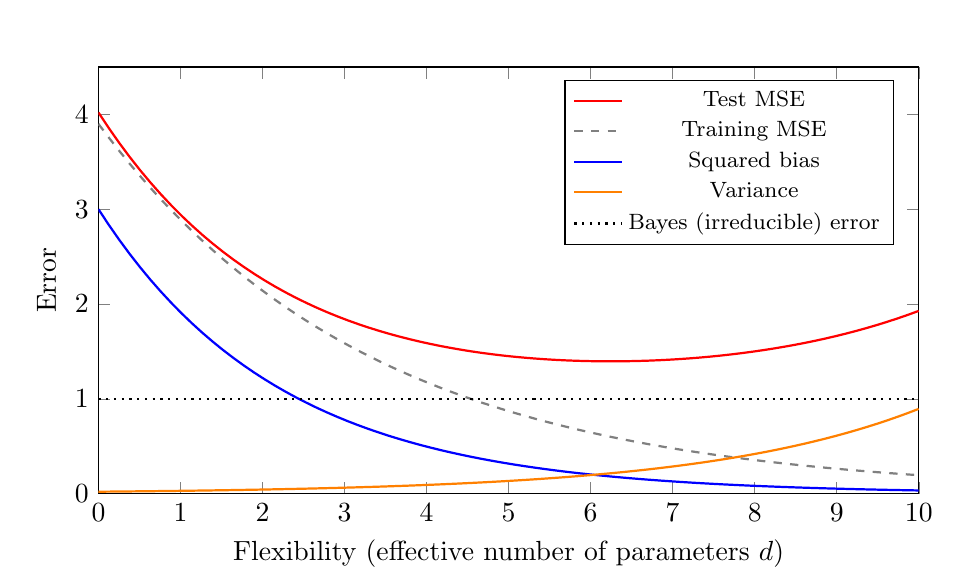
\begin{tikzpicture}
\begin{axis}[width=12cm,height=7cm,xmin=0,xmax=10,ymin=0,ymax=4.5,
  xlabel={Flexibility (effective number of parameters $d$)},ylabel={Error},
  legend pos=north east,legend style={font=\footnotesize},samples=80,domain=0:10]
\addplot[thick,red] {1+3*exp(-0.45*x)+0.02*exp(0.38*x)}; \addlegendentry{Test MSE}
\addplot[thick,gray,dashed] {3.9*exp(-0.3*x)}; \addlegendentry{Training MSE}
\addplot[thick,blue] {3*exp(-0.45*x)}; \addlegendentry{Squared bias}
\addplot[thick,orange] {0.02*exp(0.38*x)}; \addlegendentry{Variance}
\addplot[thick,black,dotted] {1}; \addlegendentry{Bayes (irreducible) error}
\end{axis}
\end{tikzpicture}
\caption{ISLP 2.3(a): the five curves as flexibility grows (illustrative functional forms).}\label{fig:I23}
\end{figure}

\passo{(b) squared bias}{Decreasing: a more flexible class of functions contains (or gets
closer to) the true $f$, so the systematic error of the fit falls, quickly at first and then
slowly once $f$ is captured.}

\passo{(b) variance}{Increasing: by \eqref{eq:I21-avgvar} of Question~1, the average variance
of a least-squares fit is $\sigma^2 d/n$, rising with $d$; a flexible fit changes a lot when one
training point changes.}

\passo{(b) irreducible error}{Flat at $\sigma^2$: it is the variance of $\epsilon$, which no
choice of $\hat f$ can predict. It is a floor for the test error in \eqref{eq:I23-sum}.}

\passo{(b) test error}{U-shaped: it is the vertical sum \eqref{eq:I23-sum}. At low flexibility
the falling bias dominates, at high flexibility the rising variance dominates, so the minimum is
at an intermediate $d$, and the curve never goes below $\sigma^2$.}

\passo{(b) training error}{Monotonically decreasing, and below the test error: the fit is chosen
to make it small, and each extra parameter can only lower it. For a correctly specified
least-squares fit with $d$ parameters,
\begin{equation}\label{eq:I23-train}
E\big[\mathrm{MSE}_{\rm tr}\big]=\sigma^2\,\frac{n-d}{n},
\end{equation}
which falls below $\sigma^2$ as $d$ grows and reaches $0$ at $d=n$ (interpolation). The gap
between test and training error is the optimism that cross-validation corrects.}

\intuicao{Training error rewards fitting the sample; test error rewards fitting the population.
Because the noise in the sample is fitted as if it were signal, the two curves separate as
flexibility grows.}
\refbib{ISLP §2.2.1--2.2.2, Figures~2.9--2.12, pp.~28--34.}
\rubrica{
\item Five labelled curves on one plot, axis labels: 3 pts (1 pt lost per missing or unlabelled curve, at most 3).
\item Correct shapes (U-shaped test, decreasing training below test, flat Bayes, decreasing bias, increasing variance): 2 pts.
\item Explanation of each shape: 1 pt each (5 pts).
\item Training error drawn above the test error or test error below the Bayes line: max.\ 5 pts in the question.
}
\end{sol}

% -----------------------------------------------------------------------------
\questao{$k$-fold cross-validation (ISLP 5.3).}
\fonte{James, Witten, Hastie, Tibshirani \& Taylor (2023), \textit{An Introduction to Statistical
Learning with Applications in Python}, Exercise~5.3 (Section~5.4, Conceptual), p.~225. Reproduced verbatim.}

We now review $k$-fold cross-validation.
\begin{enumerate}[label=(\alph*)]
\item Explain how $k$-fold cross-validation is implemented.
\item What are the advantages and disadvantages of $k$-fold cross-validation relative to:
  \begin{enumerate}[label=\roman*.]
  \item The validation set approach?
  \item LOOCV?
  \end{enumerate}
\end{enumerate}
\resolespaco
\begin{sol}
\begin{notacao}
\item $n$: number of observations; $k\in\{2,\dots,n\}$: number of folds; $C_1,\dots,C_k$: the
  folds, a random partition of $\{1,\dots,n\}$ with sizes $n_j\approx n/k$.
\item $\hat f^{(-j)}$: the model fitted without fold $j$; $\mathrm{MSE}_j$: its error on fold $j$.
\item $\mathrm{CV}_{(k)}$: the $k$-fold estimate of the test MSE; $\rho\in[0,1]$: the correlation
  between two fold errors; $\tau^2>0$: the variance of one fold error.
\end{notacao}

\passo{(a) the algorithm}{(1) Shuffle the indices and cut them into $k$ folds of (nearly) equal
size. (2) For $j=1,\dots,k$: fit the method on the other $k-1$ folds and compute
\begin{equation}\label{eq:I53-msej}
\mathrm{MSE}_j=\frac1{n_j}\sum_{i\in C_j}\big(y_i-\hat f^{(-j)}(x_i)\big)^2 .
\end{equation}
(3) Average (ISLP eq.~5.3):
\begin{equation}\label{eq:I53-cv}
\mathrm{CV}_{(k)}=\frac1k\sum_{j=1}^k\mathrm{MSE}_j .
\end{equation}
For classification, replace the squared error in \eqref{eq:I53-msej} by the indicator
$I(y_i\neq\hat y_i)$. To choose a tuning parameter (degree, $K$), repeat with the same folds
for each candidate and pick the smallest $\mathrm{CV}_{(k)}$. Each model is trained on
\begin{equation}\label{eq:I53-size}
n_{\rm train}=n\,\frac{k-1}{k}
\end{equation}
observations.}

\passo{(b)(i) versus the validation set approach}{\emph{Advantages.} (1) Lower variance: the
validation-set estimate depends on one random split, while \eqref{eq:I53-cv} averages $k$ errors
and every observation is used once for validation. (2) Lower bias: by \eqref{eq:I53-size} with
$k=10$ and $n=100$, $n_{\rm train}=100\cdot\tfrac{9}{10}=90$, against $n/2=50$ for a half split;
a model trained on fewer points is worse, so the validation set approach overstates the test
error. \emph{Disadvantage.} $k$ fits instead of one (computational cost).}

\passo{(b)(ii) versus LOOCV}{LOOCV is \eqref{eq:I53-cv} with $k=n$. \emph{Advantages of $k$-fold.}
(1) Cost: $k$ fits instead of $n$ (except for least squares, where the shortcut ISLP eq.~5.2
gives LOOCV from one fit). (2) Lower variance: the $n$ LOOCV fits share $n-2$ observations, so
their errors are highly correlated. With equicorrelated fold errors,
\begin{equation}\label{eq:I53-var}
\mathrm{Var}\big(\mathrm{CV}_{(k)}\big)=\frac{\tau^2}{k}\big(1+(k-1)\rho\big),
\end{equation}
and as $\rho\to1$ \eqref{eq:I53-var} tends to $\tau^2$: averaging nearly identical errors does
not reduce variance. \emph{Disadvantage of $k$-fold.} More bias: by \eqref{eq:I53-size} it
trains on $n(k-1)/k$ rather than $n-1$ points (e.g.\ $90$ versus $99$ for $n=100$), so it
slightly overstates the test error. $k=5$ or $10$ is the usual compromise.}

\intuicao{The three methods trade the bias of training on fewer points against the variance of
the estimate. The validation set is cheap but noisy and pessimistic; LOOCV is almost unbiased
but its $n$ near-identical fits make it noisy; $k$-fold sits in between.}
\refbib{ISLP §5.1.1--5.1.4, pp.~202--209; MS §8.6, Nota~1 (pp.~285--287); AME §1.5.1 (pp.~14--21).}
\rubrica{
\item (a) Partition, fit on $k-1$ folds, error on the held-out fold, average \eqref{eq:I53-cv}: 4 pts.
\item (b)(i) Variance and bias advantages plus the cost: 3 pts.
\item (b)(ii) Cost, variance (correlated fits) and bias: 3 pts.
\item Claiming LOOCV has \emph{higher} bias than $k$-fold: max.\ 1 pt in (b)(ii).
}
\end{sol}

% -----------------------------------------------------------------------------
\questao{Validation-set error of a logistic regression on \texttt{Default} (ISLP 5.5).}
\fonte{James, Witten, Hastie, Tibshirani \& Taylor (2023), \textit{An Introduction to Statistical
Learning with Applications in Python}, Exercise~5.5 (Section~5.4, Applied), pp.~225--226. Reproduced verbatim.}

In Chapter~4, we used logistic regression to predict the probability of \texttt{default} using
\texttt{income} and \texttt{balance} on the \texttt{Default} data set. We will now estimate the test
error of this logistic regression model using the validation set approach. Do not forget to set
a random seed before beginning your analysis.
\begin{enumerate}[label=(\alph*)]
\item Fit a logistic regression model that uses \texttt{income} and \texttt{balance} to predict \texttt{default}.
\item Using the validation set approach, estimate the test error of this model. In order to do
this, you must perform the following steps:
  \begin{enumerate}[label=\roman*.]
  \item Split the sample set into a training set and a validation set.
  \item Fit a multiple logistic regression model using only the training observations.
  \item Obtain a prediction of default status for each individual in the validation set by
  computing the posterior probability of default for that individual, and classifying the
  individual to the \texttt{default} category if the posterior probability is greater than 0.5.
  \item Compute the validation set error, which is the fraction of the observations in the
  validation set that are misclassified.
  \end{enumerate}
\item Repeat the process in (b) three times, using three different splits of the observations
into a training set and a validation set. Comment on the results obtained.
\item Now consider a logistic regression model that predicts the probability of \texttt{default}
using \texttt{income}, \texttt{balance}, and a dummy variable for \texttt{student}. Estimate the test
error for this model using the validation set approach. Comment on whether or not including a
dummy variable for \texttt{student} leads to a reduction in the test error rate.
\end{enumerate}
\resolespaco
\begin{sol}
\begin{notacao}
\item $Y_i\in\{0,1\}$: default indicator ($1=$ \texttt{Yes}); $X_{1}$: \texttt{income} (USD);
  $X_{2}$: \texttt{balance} (USD); $X_3\in\{0,1\}$: \texttt{student}; $n=10{,}000$.
\item $p(x)=\Pr(Y=1\mid X=x)\in(0,1)$; $\beta_0,\beta_1,\beta_2,\beta_3$: logistic coefficients.
\item $T,V$: training and validation index sets, $|T|=|V|=5000$; $s$: the seed of
  \texttt{numpy}'s \texttt{default\_rng(s)}, whose \texttt{permutation} defines the split.
\item $\mathrm{Err}_V$: validation error rate.
\end{notacao}

\passo{model and rule}{The multiple logistic model (ISLP eq.~4.7) is
\begin{equation}\label{eq:I55-model}
p(x)=\frac{e^{\beta_0+\beta_1x_1+\beta_2x_2}}{1+e^{\beta_0+\beta_1x_1+\beta_2x_2}},
\end{equation}
the classification rule is
\begin{equation}\label{eq:I55-rule}
\hat y=1 \iff \hat p(x)>0.5,
\end{equation}
and the validation error is
\begin{equation}\label{eq:I55-err}
\mathrm{Err}_V=\frac1{|V|}\sum_{i\in V}I(y_i\neq\hat y_i).
\end{equation}}

\passo{(a) full-sample fit}{Maximum likelihood on all $10{,}000$ observations gives
$\hat\beta_0=-11.5405$, $\hat\beta_1=2.0809\times10^{-5}$ (s.e.\ $4.985\times10^{-6}$),
$\hat\beta_2=5.6471\times10^{-3}$ (s.e.\ $2.274\times10^{-4}$). Both slopes are significant
($z=4.17$ and $24.84$). In odds terms, an extra 100 dollars of balance multiplies the odds of
default by
\begin{equation}\label{eq:I55-or}
e^{100\hat\beta_2}=e^{100\,(0.0056471)}=e^{0.56471}=1.7589 .
\end{equation}}

\passo{(b) one split ($s=1$)}{Fit \eqref{eq:I55-model} on $T$, classify $V$ with
\eqref{eq:I55-rule}. Confusion matrix on $V$ (rows: predicted; columns: true):
\begin{center}\begin{tabular}{lcc}\toprule
 & true No & true Yes\\\midrule
predicted No & 4813 & 110\\
predicted Yes & 22 & 55\\\bottomrule\end{tabular}\end{center}
The misclassified are the off-diagonal cells, $110+22=132$, so by \eqref{eq:I55-err}
\begin{equation}\label{eq:I55-b}
\mathrm{Err}_V=\frac{132}{5000}=0.0264 .
\end{equation}}

\passo{(c) three more splits}{Seeds $s=2,3,4$ give $\mathrm{Err}_V=0.0256$, $0.0296$, $0.0264$.
Averaging with \eqref{eq:I55-b}:
\begin{equation}\label{eq:I55-c}
\overline{\mathrm{Err}}=\frac{0.0264+0.0256+0.0296+0.0264}{4}=\frac{0.1080}{4}=0.0270 .
\end{equation}
The estimate moves by $0.0296-0.0256=0.0040$ across splits: the validation set approach is
noisy because it depends on which 5000 people land in $V$. All values are below the error of
the null classifier that always predicts No, $0.0333$ (the default rate).}

\passo{(d) adding \texttt{student}}{With $X_3$ in \eqref{eq:I55-model} and the same four splits:
$0.0270$, $0.0264$, $0.0294$, $0.0264$, so
\begin{equation}\label{eq:I55-d}
\overline{\mathrm{Err}}_{\rm student}=\frac{0.0270+0.0264+0.0294+0.0264}{4}=\frac{0.1092}{4}=0.0273 .
\end{equation}
Comparing \eqref{eq:I55-d} with \eqref{eq:I55-c}, the dummy does not reduce the test error: the
difference, $0.0003$, is an order of magnitude smaller than the split-to-split range $0.0040$.
Given \texttt{balance}, \texttt{student} carries little extra information for classification.}

\begin{lstlisting}
dflt = pd.read_csv("data/Default.csv"); y = (dflt.default == "Yes").astype(int).to_numpy()
X = dflt[["income", "balance"]].to_numpy()
for s in (1, 2, 3, 4):
    idx = np.random.default_rng(s).permutation(len(y)); tr, va = idx[:5000], idx[5000:]
    res = sm.Logit(y[tr], sm.add_constant(X[tr])).fit(disp=0)
    err = ((res.predict(sm.add_constant(X[va])) > 0.5) != y[va]).mean()
\end{lstlisting}

\intuicao{The error rate is dominated by the rare defaulters; whether 10 more of them fall in
the validation half moves the estimate as much as any change of model. Comparing models on a
single split is fragile; that is why ISLP moves on to LOOCV and $k$-fold CV.}
\refbib{ISLP §5.1.1 (validation set approach, pp.~202--204); §4.3.3--4.3.4 (multiple logistic regression, \texttt{Default}, pp.~141--144).}
\rubrica{
\item (a) Fit and report the coefficients: 2 pts.
\item (b) Split, train-only fit, threshold 0.5, misclassification rate: 3 pts.
\item (c) Three other splits and a comment on split variability: 2 pts.
\item (d) Model with \texttt{student}, comparison relative to the split noise: 3 pts.
\item Error computed on the training set instead of $V$: max.\ 4 pts in the question.
}
\end{sol}

% -----------------------------------------------------------------------------
\questao{LOOCV for the polynomial degree on simulated data (ISLP 5.8).}
\fonte{James, Witten, Hastie, Tibshirani \& Taylor (2023), \textit{An Introduction to Statistical
Learning with Applications in Python}, Exercise~5.8 (Section~5.4, Applied), p.~227. Reproduced verbatim.}

We will now perform cross-validation on a simulated data set.
\begin{enumerate}[label=(\alph*)]
\item Generate a simulated data set as follows:
\begin{lstlisting}[frame=none]
rng = np.random.default_rng(1)
x = rng.normal(size=100)
y = x - 2 * x**2 + rng.normal(size=100)
\end{lstlisting}
In this data set, what is $n$ and what is $p$? Write out the model used to generate the data in equation form.
\item Create a scatterplot of $X$ against $Y$. Comment on what you find.
\item Set a random seed, and then compute the LOOCV errors that result from fitting the following four models using least squares:
  \begin{enumerate}[label=\roman*.]
  \item $Y=\beta_0+\beta_1X+\epsilon$
  \item $Y=\beta_0+\beta_1X+\beta_2X^2+\epsilon$
  \item $Y=\beta_0+\beta_1X+\beta_2X^2+\beta_3X^3+\epsilon$
  \item $Y=\beta_0+\beta_1X+\beta_2X^2+\beta_3X^3+\beta_4X^4+\epsilon$.
  \end{enumerate}
  Note you may find it helpful to use the \texttt{data.frame()} function to create a single data set containing both $X$ and $Y$.
\item Repeat (c) using another random seed, and report your results. Are your results the same as what you got in (c)? Why?
\item Which of the models in (c) had the smallest LOOCV error? Is this what you expected? Explain your answer.
\item Comment on the statistical significance of the coefficient estimates that results from
fitting each of the models in (c) using least squares. Do these results agree with the
conclusions drawn based on the cross-validation results?
\end{enumerate}
\resolespaco
\begin{sol}
\begin{notacao}
\item $X_i\sim N(0,1)$, $\epsilon_i\sim N(0,1)$ independent, $i=1,\dots,n$; $Y_i$: response.
\item $m\in\{1,2,3,4\}$: polynomial degree of model i--iv; $\mathbf X_m$: the $n\times(m+1)$ matrix with columns $1,X,\dots,X^m$.
\item $\mathbf H_m=\mathbf X_m(\mathbf X_m'\mathbf X_m)^{-1}\mathbf X_m'$; $h_i$: its $i$-th diagonal element (leverage), $1/n\le h_i\le1$.
\item $\hat y_i$: full-sample fitted value; $\mathrm{CV}_{(n)}$: LOOCV estimate of the test MSE.
\end{notacao}

\passo{(a) $n$, $p$ and the model}{$n=100$ observations and $p=1$ predictor ($X$; the model
uses $X$ and $X^2$, but both are functions of one variable). The data-generating process is
\begin{equation}\label{eq:I58-dgp}
Y=X-2X^2+\epsilon,\qquad X\sim N(0,1),\ \epsilon\sim N(0,1),
\end{equation}
i.e.\ model ii with $\beta_0=0$, $\beta_1=1$, $\beta_2=-2$ and $\sigma^2=1$.}

\passo{(b) the scatterplot}{Figure~\ref{fig:I58} shows an inverted parabola. From
\eqref{eq:I58-dgp}, $E(Y\mid X=x)=x-2x^2$; setting its derivative to zero,
\begin{equation}\label{eq:I58-foc}
1-4x=0\ \Rightarrow\ x=0.25,
\end{equation}
and substituting \eqref{eq:I58-foc} into \eqref{eq:I58-dgp}, the peak is
$0.25-2(0.25)^2=0.25-0.125=0.125$. The sample $y$ ranges from $-14.864$ to $2.097$: the
quadratic term makes large $|x|$ produce very negative $y$, so a straight line cannot fit.}

\begin{figure}[h]\centering
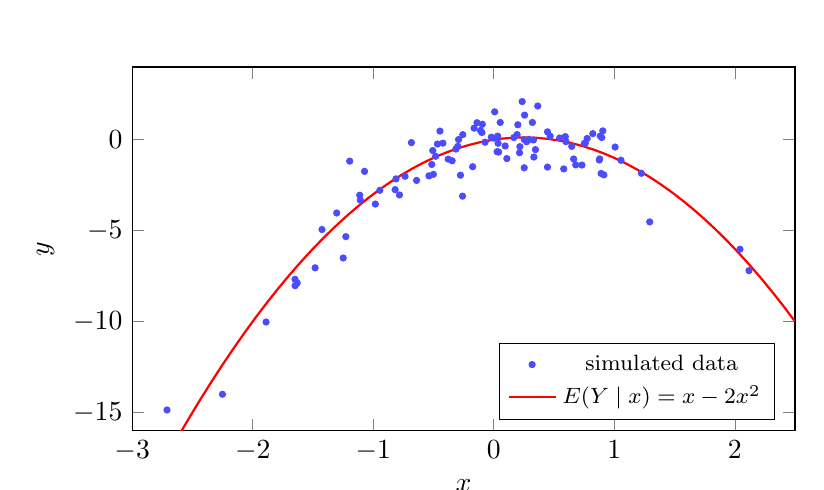
\begin{tikzpicture}
\begin{axis}[width=10cm,height=6.2cm,xlabel={$x$},ylabel={$y$},xmin=-3,xmax=2.5,ymin=-16,ymax=4,
  legend pos=south east,legend style={font=\footnotesize}]
\addplot[only marks,mark=*,mark size=1.1pt,blue!70] coordinates {(0.346,-0.545) (0.822,0.334) (0.330,-0.014) (-1.303,-4.030) (0.905,0.485) (0.446,0.431) (-0.537,-1.989) (0.581,-1.609) (0.365,1.852) (0.294,0.010) (0.028,-0.662) (0.547,0.093) (-0.736,-2.013) (-0.163,0.636) (-0.482,-0.913) (0.599,-0.105) (0.040,-0.678) (-0.292,0.006) (-0.782,-3.039) (-0.257,0.276) (0.008,1.532) (-0.276,-1.952) (1.294,-4.521) (1.007,-0.403) (-2.711,-14.864) (-1.889,-10.027) (-0.175,-1.487) (-0.422,-0.190) (0.214,-0.718) (0.217,-0.383) (2.118,-7.201) (-1.112,-3.053) (-0.378,-1.068) (2.043,-6.025) (0.647,-0.366) (0.663,-1.061) (-0.514,-1.362) (-1.648,-8.031) (0.167,0.118) (0.109,-1.039) (-1.227,-5.333) (-0.683,-0.160) (-0.072,-0.136) (-0.945,-2.784) (-0.098,0.394) (0.095,-0.344) (0.036,-0.195) (-0.506,-0.594) (0.594,0.171) (0.891,-1.856) (0.321,0.948) (-0.818,-2.748) (0.732,-1.395) (-0.501,-1.905) (0.879,-1.057) (-1.072,-1.742) (0.914,-1.934) (-0.020,0.139) (-1.249,-6.505) (-0.314,-0.513) (0.054,0.948) (0.273,-0.113) (-0.982,-3.541) (-1.107,-3.328) (0.200,0.820) (-0.467,-0.239) (0.236,2.097) (0.760,-0.185) (-1.649,-7.678) (0.254,-0.001) (1.225,-1.847) (-0.298,-0.366) (-0.811,-2.156) (0.752,-0.206) (0.253,-1.546) (0.896,0.120) (-0.345,-1.158) (-1.482,-7.047) (-0.110,0.504) (-0.446,0.474) (0.775,0.066) (0.194,0.280) (-1.631,-7.882) (-1.195,-1.180) (0.884,0.202) (0.680,-1.384) (-0.640,-2.240) (-0.001,0.086) (0.446,-1.506) (0.468,0.198) (0.876,-1.118) (0.256,1.351) (-0.095,0.849) (-0.259,-3.104) (1.056,-1.132) (-2.251,-14.001) (-0.139,0.933) (0.033,0.199) (-1.425,-4.940) (0.333,-0.954)};
\addlegendentry{simulated data}
\addplot[thick,red,domain=-3:2.5,samples=60] {x-2*x^2}; \addlegendentry{$E(Y\mid x)=x-2x^2$}
\end{axis}
\end{tikzpicture}
\caption{ISLP 5.8(b): the 100 simulated points and the true regression function.}\label{fig:I58}
\end{figure}

\passo{(c) LOOCV errors}{For least squares, LOOCV has the closed form (ISLP eq.~5.2)
\begin{equation}\label{eq:I58-cv}
\mathrm{CV}_{(n)}=\frac1n\sum_{i=1}^n\left(\frac{y_i-\hat y_i}{1-h_i}\right)^2 ,
\end{equation}
with $h_i$ the diagonal of $\mathbf H_m$. Evaluating \eqref{eq:I58-cv} (and checking it against
100 explicit leave-one-out fits, which agree to $10^{-10}$):
\begin{center}\begin{tabular}{lcccc}\toprule
model & i ($m=1$) & ii ($m=2$) & iii ($m=3$) & iv ($m=4$)\\\midrule
$\mathrm{CV}_{(n)}$ & 6.6330 & 1.1229 & 1.3018 & 1.3324\\\bottomrule\end{tabular}\end{center}}

\passo{(d) another seed}{The results are identical. LOOCV leaves out each observation exactly
once, so \eqref{eq:I58-cv} is a deterministic function of the data; there is no random split for
the seed to change (the data themselves were fixed in (a)).}

\passo{(e) the smallest error}{Model ii, $\mathrm{CV}_{(n)}=1.1229$. This is expected: by
\eqref{eq:I58-dgp} the truth is quadratic, so model i has a large bias (6.6330), and models
iii--iv add terms whose true coefficients are zero, which only adds variance. For a correctly
specified model with $m+1$ coefficients the expected test MSE is about
$\sigma^2\big(1+\tfrac{m+1}{n}\big)=1\cdot\big(1+\tfrac{3}{100}\big)=1.03$, close to $1.1229$.}

\passo{(f) significance}{OLS $t$-statistics (and $p$-values) on the full sample:
\begin{center}\begin{tabular}{lccccc}\toprule
model & $\hat\beta_0$ & $\hat\beta_1$ & $\hat\beta_2$ & $\hat\beta_3$ & $\hat\beta_4$\\\midrule
i   & $-5.94$ (0.000) & $6.75$ (0.000) & & & \\
ii  & $-0.61$ (0.543) & $7.65$ (0.000) & $-22.07$ (0.000) & & \\
iii & $-0.48$ (0.635) & $5.95$ (0.000) & $-20.67$ (0.000) & $-1.07$ (0.287) & \\
iv  & $0.74$ (0.460) & $4.42$ (0.000) & $-11.34$ (0.000) & $0.47$ (0.642) & $2.31$ (0.023)\\\bottomrule\end{tabular}\end{center}
The linear and quadratic terms are always highly significant; the cubic term never is. The
quartic term has $p=0.023$, which by itself would suggest model iv, but LOOCV rejects it
($1.3324>1.1229$). This is a false positive of the kind expected when many coefficients are
tested at 5\%, helped by the extreme $x$ values (the largest leverage is $h_i=0.836$ in model
iv), which a fourth power fits closely. Overall the tests and CV agree on model ii; where they
disagree, CV measures what matters for prediction.}

\begin{lstlisting}
for m in (1, 2, 3, 4):
    B = np.column_stack([x**j for j in range(m + 1)])
    H = B @ np.linalg.solve(B.T @ B, B.T)
    cv = np.mean(((y - H @ y) / (1 - np.diag(H)))**2)       # (5.2)
    fit = sm.OLS(y, B).fit()                                  # t-stats, p-values for (f)
\end{lstlisting}

\intuicao{LOOCV estimates out-of-sample error directly, so it penalizes the extra variance of
superfluous terms automatically, while each $t$-test asks only whether one coefficient is zero.}
\refbib{ISLP §5.1.2 (LOOCV and eq.~5.2, pp.~204--206); §3.3.2 (non-linear relationships, p.~98).}
\rubrica{
\item (a) $n=100$, $p=1$, model \eqref{eq:I58-dgp}: 1 pt. (b) plot and comment: 1 pt.
\item (c) four LOOCV errors: 3 pts. (d) identical, with the reason: 1.5 pts.
\item (e) model ii and why: 1.5 pts. (f) significance and its relation to CV: 2 pts.
\item Saying the results change with the seed in (d): max.\ 0.5 pt in (d).
}
\end{sol}

% -----------------------------------------------------------------------------
\questao{CV-chosen polynomial degree and step functions for \texttt{Wage} (ISLP 7.6).}
\fonte{James, Witten, Hastie, Tibshirani \& Taylor (2023), \textit{An Introduction to Statistical
Learning with Applications in Python}, Exercise~7.6 (Section~7.9, Applied), p.~327. Reproduced verbatim.}

In this exercise, you will further analyze the \texttt{Wage} data set considered throughout this chapter.
\begin{enumerate}[label=(\alph*)]
\item Perform polynomial regression to predict \texttt{wage} using \texttt{age}. Use
cross-validation to select the optimal degree $d$ for the polynomial. What degree was chosen,
and how does this compare to the results of hypothesis testing using ANOVA? Make a plot of the
resulting polynomial fit to the data.
\item Fit a step function to predict \texttt{wage} using \texttt{age}, and perform
cross-validation to choose the optimal number of cuts. Make a plot of the fit obtained.
\end{enumerate}
\resolespaco
\begin{sol}
\begin{notacao}
\item $y_i$: \texttt{wage} (thousands of USD); $x_i$: \texttt{age} (18--80 years); $n=3000$.
\item $d\in\{1,\dots,10\}$: polynomial degree; $\mathrm{RSS}_d$: residual sum of squares of the
  degree-$d$ fit; $\mathrm{CV}_{(10)}(d)$: 10-fold CV estimate of the test MSE.
\item $c\in\{2,\dots,10\}$: number of intervals of the step function ($c-1$ cut points), equal
  width over $[18,80]$; $C_1(x),\dots,C_{c-1}(x)$: interval dummies (the first interval is the base).
\item Folds: \texttt{numpy.random.default\_rng(1).permutation(n) \% 10}, the same for every model.
\end{notacao}

\passo{model and criterion}{The polynomial regression (ISLP eq.~7.1) is
\begin{equation}\label{eq:I76-poly}
y_i=\beta_0+\beta_1x_i+\beta_2x_i^2+\dots+\beta_dx_i^d+\epsilon_i ,
\end{equation}
fitted by least squares (with $x$ standardized before taking powers, which changes no fitted
value but avoids ill-conditioning). For each $d$ the 10-fold CV error is \eqref{eq:I53-cv} of
Question~3 with $k=10$.}

\passo{(a) CV choice}{The 10-fold CV errors are:
\begin{center}\small\setlength{\tabcolsep}{3.5pt}\begin{tabular}{lcccccccccc}\toprule
$d$ & 1 & 2 & 3 & 4 & 5 & 6 & 7 & 8 & 9 & 10\\\midrule
$\mathrm{CV}_{(10)}$ & 1675.48 & 1599.65 & 1594.81 & 1593.32 & 1593.23 & 1592.32 & 1592.06 & 1592.70 & 1590.97 & 1592.11\\\bottomrule\end{tabular}\end{center}
The minimum is at $d=9$ (repeating the CV with fold seeds $2,\dots,5$, the minimum is at $d=6$
for seed 2 and at $d=9$ for seeds 3, 4 and 5). But the curve is flat beyond $d=3$--4:
the gain from $d=4$ to $d=9$ is
\begin{equation}\label{eq:I76-gain}
1593.32-1590.97=2.35,\qquad \frac{2.35}{1593.32}=0.0015,
\end{equation}
a $0.15\%$ reduction, far inside the sampling noise of a CV estimate. The big step is from
$d=1$ to $d=2$ (75.83), with a small further gain to $d=3$.}

\passo{(a) ANOVA}{Nested $F$-tests compare degree $d-1$ with $d$, using the residual variance of
the largest model ($d=5$), as \texttt{anova\_lm} does:
\begin{equation}\label{eq:I76-F}
F_d=\frac{\mathrm{RSS}_{d-1}-\mathrm{RSS}_d}{\mathrm{RSS}_5/(n-6)},\qquad F_d\sim F_{1,\,n-6}\ \text{under } H_0:\beta_d=0 .
\end{equation}
The denominator of \eqref{eq:I76-F} is
\begin{equation}\label{eq:I76-s2}
\frac{\mathrm{RSS}_5}{n-6}=\frac{4770321.69}{3000-6}=\frac{4770321.69}{2994}=1593.29 .
\end{equation}
Substituting \eqref{eq:I76-s2} into \eqref{eq:I76-F}, e.g.\ for $d=3$:
\begin{equation}\label{eq:I76-F3}
F_3=\frac{4793430.09-4777674.40}{1593.29}=\frac{15755.69}{1593.29}=9.889 .
\end{equation}
All four comparisons:
\begin{center}\small\begin{tabular}{lccc}\toprule
comparison & $\mathrm{RSS}_{d-1}-\mathrm{RSS}_d$ & $F_d$ & $p$-value\\\midrule
$d=1\to2$ & $5022216.10-4793430.09=228786.01$ & 143.59 & $<0.001$\\
$d=2\to3$ & $4793430.09-4777674.40=15755.69$ & 9.889 & 0.0017\\
$d=3\to4$ & $4777674.40-4771604.25=6070.15$ & 3.810 & 0.0510\\
$d=4\to5$ & $4771604.25-4770321.69=1282.56$ & 0.805 & 0.3697\\\bottomrule\end{tabular}\end{center}
ANOVA keeps the cubic (and the quartic at the 10\% level only) and rejects $d=5$. CV and ANOVA
agree on what matters: degree 1 and 2 are clearly too rigid and nothing beyond $d\approx 4$ buys
a material improvement; CV's literal minimizer $d=9$ is within noise of $d=3$--4. A
parsimonious choice is $d=4$, plotted in Figure~\ref{fig:I76}:
\begin{equation}\label{eq:I76-fit4}
\widehat{\texttt{wage}}=-184.154+21.2455\,x-0.563859\,x^2+0.00681069\,x^3-0.0000320383\,x^4,
\end{equation}
which peaks at age $48.35$.}

\passo{(b) step function}{The step-function model (ISLP eq.~7.5) is
\begin{equation}\label{eq:I76-step}
y_i=\beta_0+\beta_1C_1(x_i)+\dots+\beta_{c-1}C_{c-1}(x_i)+\epsilon_i ,
\end{equation}
whose fit is the mean wage within each interval. With interval edges fixed on the full range
$[18,80]$ and the same folds:
\begin{center}\small\setlength{\tabcolsep}{3.5pt}\begin{tabular}{lccccccccc}\toprule
$c$ & 2 & 3 & 4 & 5 & 6 & 7 & 8 & 9 & 10\\\midrule
$\mathrm{CV}_{(10)}$ & 1733.16 & 1681.80 & 1634.27 & 1629.82 & 1621.38 & 1609.87 & 1599.57 & 1607.75 & 1602.75\\\bottomrule\end{tabular}\end{center}
CV selects $c=8$ intervals (7 cuts), with edges $18, 25.75, 33.5, 41.25, 49, 56.75, 64.5, 72.25, 80$
and fitted levels $76.28, 102.12, 116.51, 119.78, 116.42, 120.38, 105.23, 91.51$. Even the best
step function ($1599.57$) does worse than the cubic ($1594.81$): the steps cannot follow the
smooth rise of wages in the 20s.}

\begin{figure}[h]\centering
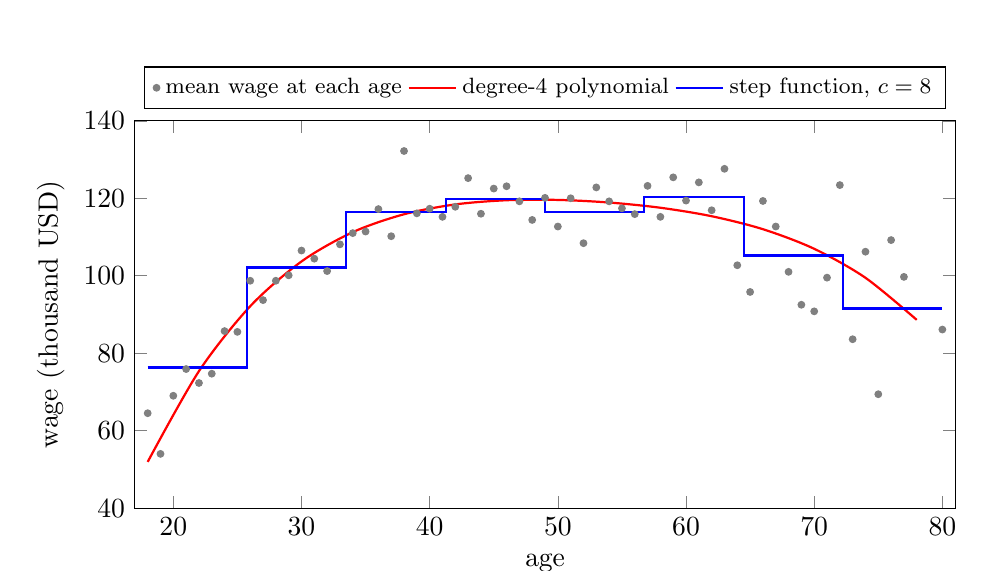
\begin{tikzpicture}
\begin{axis}[width=12cm,height=6.5cm,xlabel={age},ylabel={wage (thousand USD)},xmin=17,xmax=81,ymin=40,ymax=140,
  legend style={font=\footnotesize,at={(0.5,1.03)},anchor=south},legend columns=3]
\addplot[only marks,mark=*,mark size=1.2pt,gray] coordinates {(18,64.5) (19,54.0) (20,69.0) (21,75.9) (22,72.3) (23,74.7) (24,85.7) (25,85.5) (26,98.7) (27,93.7) (28,98.7) (29,100.1) (30,106.5) (31,104.4) (32,101.2) (33,108.1) (34,111.0) (35,111.4) (36,117.2) (37,110.2) (38,132.2) (39,116.1) (40,117.3) (41,115.2) (42,117.8) (43,125.2) (44,116.0) (45,122.5) (46,123.1) (47,119.2) (48,114.4) (49,120.1) (50,112.7) (51,120.0) (52,108.4) (53,122.8) (54,119.2) (55,117.4) (56,115.9) (57,123.2) (58,115.2) (59,125.4) (60,119.4) (61,124.1) (62,116.9) (63,127.6) (64,102.7) (65,95.8) (66,119.3) (67,112.7) (68,101.0) (69,92.5) (70,90.8) (71,99.5) (72,123.4) (73,83.6) (74,106.2) (75,69.4) (76,109.2) (77,99.7) (80,86.1)};
\addlegendentry{mean wage at each age}
\addplot[thick,red,smooth] coordinates {(18,51.93) (22,75.35) (26,92.12) (30,103.68) (34,111.25) (38,115.87) (42,118.41) (46,119.49) (50,119.57) (54,118.90) (58,117.55) (62,115.36) (66,112.01) (70,106.95) (74,99.46) (78,88.60)};
\addlegendentry{degree-4 polynomial}
\addplot[thick,blue,const plot] coordinates {(18,76.28) (25.75,102.12) (33.5,116.51) (41.25,119.78) (49,116.42) (56.75,120.38) (64.5,105.23) (72.25,91.51) (80,91.51)};
\addlegendentry{step function, $c=8$}
\end{axis}
\end{tikzpicture}
\caption{ISLP 7.6: polynomial and step-function fits (the 3000 points are summarized by the mean wage at each age).}\label{fig:I76}
\end{figure}

\begin{lstlisting}
wage = pd.read_csv("data/Wage.csv"); age, wg = wage.age.to_numpy(float), wage.wage.to_numpy()
basis = lambda a, d: np.column_stack([((a - age.mean()) / age.std())**j for j in range(d + 1)])
cv = {d: cv_mse(lambda a: basis(a, d), age, wg, k=10, seed=1) for d in range(1, 11)}
edges = np.linspace(18, 80, c + 1)                         # step function with c intervals
step = lambda a: np.column_stack([np.ones(len(a))] + [((a > edges[j]) & (a <= edges[j+1]))
                                  .astype(float) for j in range(1, c)])
\end{lstlisting}

\intuicao{Wages rise steeply until the mid-30s, flatten, and fall after 60. Three to four
polynomial terms capture this shape; more terms only wiggle around it, which CV can barely
distinguish from no change. Step functions pay a bias price for being flat inside each bin.}
\refbib{ISLP §7.1--7.2 (pp.~290--293), §7.8.1 lab (ANOVA for the polynomial degree, p.~310); §5.1.3 ($k$-fold CV, p.~206).}
\rubrica{
\item (a) CV over degrees with the table and the selected degree: 3 pts; ANOVA $F$-tests and comparison: 2 pts; plot: 1 pt.
\item (b) Step function, CV over the number of cuts, selected value: 3 pts; plot: 1 pt.
\item Choosing the degree by training RSS (always the largest $d$): max.\ 2 pts in (a).
}
\end{sol}

% -----------------------------------------------------------------------------
\questao{Polynomials and regression splines for \texttt{nox} on \texttt{dis} (ISLP 7.9).}
\fonte{James, Witten, Hastie, Tibshirani \& Taylor (2023), \textit{An Introduction to Statistical
Learning with Applications in Python}, Exercise~7.9 (Section~7.9, Applied), p.~327. Reproduced verbatim.}

This question uses the variables \texttt{dis} (the weighted mean of distances to five Boston
employment centers) and \texttt{nox} (nitrogen oxides concentration in parts per 10 million) from
the \texttt{Boston} data. We will treat \texttt{dis} as the predictor and \texttt{nox} as the response.
\begin{enumerate}[label=(\alph*)]
\item Use the \texttt{poly()} function from the \texttt{ISLP.models} module to fit a cubic
polynomial regression to predict \texttt{nox} using \texttt{dis}. Report the regression output, and
plot the resulting data and polynomial fits.
\item Plot the polynomial fits for a range of different polynomial degrees (say, from 1 to 10),
and report the associated residual sum of squares.
\item Perform cross-validation or another approach to select the optimal degree for the
polynomial, and explain your results.
\item Use the \texttt{bs()} function from the \texttt{ISLP.models} module to fit a regression
spline to predict \texttt{nox} using \texttt{dis}. Report the output for the fit using four degrees
of freedom. How did you choose the knots? Plot the resulting fit.
\item Now fit a regression spline for a range of degrees of freedom, and plot the resulting fits
and report the resulting RSS. Describe the results obtained.
\item Perform cross-validation or another approach in order to select the best degrees of
freedom for a regression spline on this data. Describe your results.
\end{enumerate}
\resolespaco
\begin{sol}
\begin{notacao}
\item $y_i$: \texttt{nox} (parts per 10 million); $x_i$: \texttt{dis} (from 1.13 to 12.13); $n=506$.
\item $d$: polynomial degree; $\mathrm{RSS}=\sum_i(y_i-\hat y_i)^2$; $\mathrm{CV}_{(10)}$: 10-fold
  CV error, folds from \texttt{default\_rng(1)}, identical for every model.
\item $\xi_1<\dots<\xi_K$: interior knots of a cubic spline; $\mathrm{df}$: number of spline basis
  columns excluding the intercept; $B_j(x)$: cubic B-spline basis functions.
\end{notacao}

\passo{(a) cubic fit}{Least squares on $1,x,x^2,x^3$ (\texttt{poly()} uses an orthogonal basis by
default; the fitted values, $R^2$ and RSS are the same, and the raw coefficients are easier to
read):
\begin{equation}\label{eq:I79-cubic}
\widehat{\texttt{nox}}=\underset{(0.0207)}{0.9341}-\underset{(0.0147)}{0.1821}\,x+\underset{(0.00293)}{0.02193}\,x^2-\underset{(0.000173)}{0.000885}\,x^3,
\end{equation}
standard errors in parentheses, every $p$-value $<0.001$, $R^2=0.7148$, $\mathrm{RSS}=1.9341$.
Figure~\ref{fig:I79} plots the data and \eqref{eq:I79-cubic}: \texttt{nox} falls steeply as
distance grows up to about 6 and then levels off; the cubic bends down again at the right edge,
where data are sparse.}

\passo{(b) degrees 1 to 10}{Residual sums of squares:
\begin{center}\small\setlength{\tabcolsep}{3.5pt}\begin{tabular}{lcccccccccc}\toprule
$d$ & 1 & 2 & 3 & 4 & 5 & 6 & 7 & 8 & 9 & 10\\\midrule
RSS & 2.7686 & 2.0353 & 1.9341 & 1.9330 & 1.9153 & 1.8783 & 1.8495 & 1.8356 & 1.8333 & 1.8322\\\bottomrule\end{tabular}\end{center}
RSS falls monotonically because the models are nested (each adds one column): training error
cannot rise with flexibility (Question~2). The drop is large up to $d=3$ and small afterwards.}

\passo{(c) CV for the degree}{10-fold CV errors (multiplied by $10^3$):
\begin{center}\small\setlength{\tabcolsep}{3.5pt}\begin{tabular}{lcccccccccc}\toprule
$d$ & 1 & 2 & 3 & 4 & 5 & 6 & 7 & 8 & 9 & 10\\\midrule
$10^3\,\mathrm{CV}_{(10)}$ & 5.526 & 4.065 & 3.852 & 3.867 & 4.184 & 5.811 & 8.736 & 8.281 & 12.092 & 3.987\\\bottomrule\end{tabular}\end{center}
CV selects $d=3$. Unlike RSS, the CV error rises again for $d\ge5$ and is erratic: a high-degree
polynomial fitted without the few observations at large \texttt{dis} extrapolates wildly at
those points when they are held out. The cubic balances bias and variance.}

\passo{(d) spline with 4 df}{A cubic spline with $K$ interior knots has, excluding the intercept,
\begin{equation}\label{eq:I79-df}
\mathrm{df}=3+K
\end{equation}
basis functions. With $\mathrm{df}=4$, \eqref{eq:I79-df} gives $K=4-3=1$ knot. Knots are placed
at uniform quantiles of $x$ (the default of \texttt{bs()}), so the single knot is the median,
$\xi_1=3.2074$. The model is
\begin{equation}\label{eq:I79-bs}
y_i=\beta_0+\sum_{j=1}^{4}\beta_jB_j(x_i)+\epsilon_i ,
\end{equation}
with estimates (standard errors) $\hat\beta_0=0.7345\,(0.0146)$, $\hat\beta_1=-0.0581\,(0.0219)$,
$\hat\beta_2=-0.4636\,(0.0237)$, $\hat\beta_3=-0.1998\,(0.0431)$, $\hat\beta_4=-0.3888\,(0.0455)$;
$\mathrm{RSS}=1.9228$, $R^2=0.7164$. The B-spline coefficients have no direct meaning (each
weights a local bump); the fit (Figure~\ref{fig:I79}) is close to the cubic but bends less at the
right edge.}

\passo{(e) a range of df}{RSS of cubic regression splines:
\begin{center}\begin{tabular}{lcccccccc}\toprule
df & 3 & 4 & 5 & 6 & 7 & 8 & 9 & 10\\\midrule
RSS & 1.9341 & 1.9228 & 1.8402 & 1.8340 & 1.8299 & 1.8170 & 1.8257 & 1.7925\\\bottomrule\end{tabular}\end{center}
With $\mathrm{df}=3$, \eqref{eq:I79-df} gives $K=0$: the spline is the global cubic, and its RSS,
$1.9341$, equals the cubic RSS of (b), a useful check. RSS falls with df but not monotonically
($1.8257>1.8170$ at $\mathrm{df}=9$), because changing df moves all the quantile knots, so the
models are not nested.}

\passo{(f) CV for the df}{10-fold CV errors (multiplied by $10^3$):
\begin{center}\small\begin{tabular}{lcccccccc}\toprule
df & 3 & 4 & 5 & 6 & 7 & 8 & 9 & 10\\\midrule
$10^3\,\mathrm{CV}_{(10)}$ & 3.852 & 3.875 & 3.688 & 3.687 & 3.700 & 3.690 & 3.715 & 3.695\\\bottomrule\end{tabular}\end{center}
The minimum is at $\mathrm{df}=6$ ($0.003687$), but $\mathrm{df}=5$ to $10$ are all within $0.00003$
of it; any of them improves on the global cubic ($0.003852$), and $\mathrm{df}=5$ is the
parsimonious choice. Splines do not suffer the erratic CV of high-degree polynomials because
each basis function is local.}

\begin{figure}[h]\centering
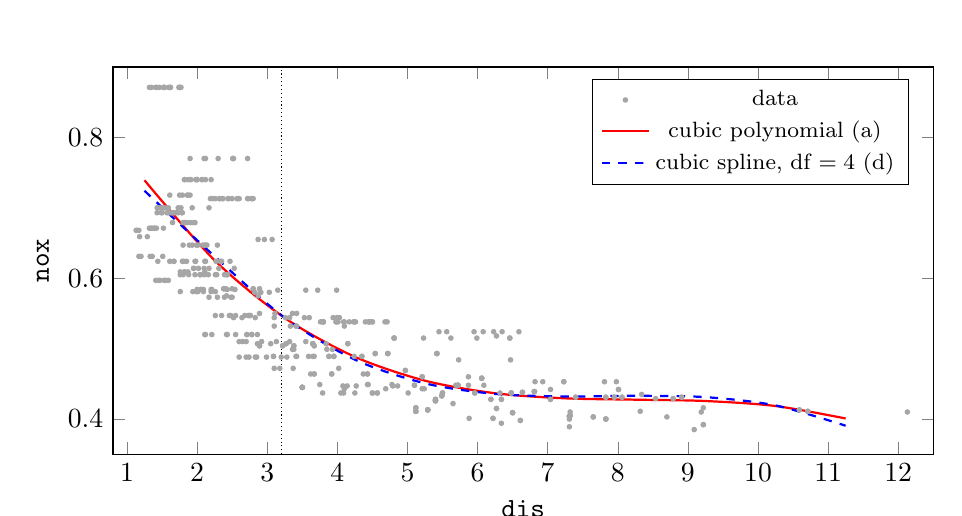
\begin{tikzpicture}
\begin{axis}[width=12cm,height=6.5cm,xlabel={\texttt{dis}},ylabel={\texttt{nox}},xmin=0.8,xmax=12.5,ymin=0.35,ymax=0.9,
  legend pos=north east,legend style={font=\footnotesize}]
\addplot[only marks,mark=*,mark size=0.8pt,gray!70] coordinates {(4.09,0.538) (4.97,0.469) (4.97,0.469) (6.06,0.458) (6.06,0.458) (6.06,0.458) (5.56,0.524) (5.95,0.524) (6.08,0.524) (6.59,0.524) (6.35,0.524) (6.23,0.524) (5.45,0.524) (4.71,0.538) (4.46,0.538) (4.50,0.538) (4.50,0.538) (4.26,0.538) (3.80,0.538) (3.80,0.538) (3.80,0.538) (4.01,0.538) (3.98,0.538) (4.10,0.538) (4.40,0.538) (4.45,0.538) (4.68,0.538) (4.45,0.538) (4.45,0.538) (4.24,0.538) (4.23,0.538) (4.17,0.538) (3.99,0.538) (3.79,0.538) (3.76,0.538) (3.36,0.499) (3.38,0.499) (3.93,0.499) (3.85,0.499) (5.40,0.428) (5.40,0.428) (5.72,0.448) (5.72,0.448) (5.72,0.448) (5.72,0.448) (5.10,0.448) (5.10,0.448) (5.69,0.448) (5.87,0.448) (6.09,0.448) (6.81,0.439) (6.81,0.439) (6.81,0.439) (6.81,0.439) (7.32,0.410) (8.70,0.403) (9.19,0.410) (8.32,0.411) (7.81,0.453) (6.93,0.453) (7.23,0.453) (6.82,0.453) (7.23,0.453) (7.98,0.453) (9.22,0.416) (6.61,0.398) (6.61,0.398) (6.50,0.409) (6.50,0.409) (6.50,0.409) (5.29,0.413) (5.29,0.413) (5.29,0.413) (5.29,0.413) (4.25,0.437) (4.50,0.437) (4.05,0.437) (4.09,0.437) (5.01,0.437) (4.50,0.437) (5.40,0.426) (5.40,0.426) (5.40,0.426) (5.40,0.426) (4.78,0.449) (4.44,0.449) (4.43,0.449) (3.75,0.449) (3.42,0.489) (3.41,0.489) (3.09,0.489) (3.09,0.489) (3.67,0.464) (3.67,0.464) (3.62,0.464) (3.50,0.445) (3.50,0.445) (3.50,0.445) (3.50,0.445) (3.50,0.445) (2.78,0.520) (2.86,0.520) (2.71,0.520) (2.71,0.520) (2.42,0.520) (2.11,0.520) (2.21,0.520) (2.12,0.520) (2.43,0.520) (2.55,0.520) (2.78,0.520) (2.68,0.547) (2.35,0.547) (2.55,0.547) (2.26,0.547) (2.46,0.547) (2.73,0.547) (2.75,0.547) (2.48,0.547) (2.76,0.547) (2.26,0.581) (2.20,0.581) (2.09,0.581) (1.94,0.581) (2.01,0.581) (1.99,0.581) (1.76,0.581) (1.79,0.624) (1.81,0.624) (1.98,0.624) (2.12,0.624) (2.27,0.624) (2.33,0.624) (2.47,0.624) (2.35,0.624) (2.11,0.624) (1.97,0.624) (1.85,0.624) (1.67,0.624) (1.67,0.624) (1.61,0.624) (1.44,0.624) (1.32,0.871) (1.41,0.871) (1.35,0.871) (1.42,0.871) (1.52,0.871) (1.46,0.871) (1.53,0.871) (1.53,0.871) (1.62,0.871) (1.59,0.871) (1.61,0.871) (1.62,0.871) (1.75,0.871) (1.75,0.871) (1.74,0.871) (1.88,0.605) (1.76,0.605) (1.77,0.871) (1.80,0.605) (1.97,0.605) (2.04,0.605) (2.16,0.605) (2.42,0.605) (2.28,0.605) (2.05,0.605) (2.43,0.605) (2.10,0.605) (2.26,0.605) (2.43,0.605) (2.39,0.605) (2.60,0.510) (2.65,0.510) (2.70,0.510) (3.13,0.510) (3.55,0.510) (3.32,0.510) (2.92,0.510) (2.83,0.488) (2.74,0.488) (2.60,0.488) (2.70,0.488) (2.85,0.488) (2.99,0.488) (3.28,0.488) (3.20,0.488) (3.79,0.437) (4.57,0.437) (4.57,0.437) (6.48,0.437) (6.48,0.437) (6.48,0.437) (6.22,0.401) (6.22,0.401) (5.65,0.422) (7.31,0.404) (7.31,0.404) (7.31,0.404) (7.65,0.403) (7.65,0.403) (6.27,0.415) (6.27,0.415) (5.12,0.416) (5.12,0.416) (3.95,0.489) (4.35,0.489) (4.35,0.489) (4.24,0.489) (3.88,0.489) (3.88,0.489) (3.67,0.489) (3.65,0.489) (3.95,0.489) (3.59,0.489) (3.95,0.489) (3.11,0.550) (3.42,0.550) (2.89,0.550) (3.36,0.550) (2.86,0.507) (3.05,0.507) (3.27,0.507) (3.27,0.507) (2.89,0.504) (2.89,0.504) (3.22,0.504) (3.22,0.504) (3.38,0.504) (3.38,0.504) (3.67,0.504) (3.67,0.504) (3.84,0.507) (3.65,0.507) (3.65,0.507) (3.65,0.507) (4.15,0.507) (4.15,0.507) (6.19,0.428) (6.19,0.428) (6.34,0.428) (6.34,0.428) (7.04,0.428) (7.04,0.428) (7.95,0.431) (7.95,0.431) (8.06,0.431) (8.06,0.431) (7.83,0.431) (7.83,0.431) (7.40,0.431) (7.40,0.431) (8.91,0.431) (8.91,0.431) (9.22,0.392) (9.22,0.392) (6.34,0.394) (1.80,0.647) (1.89,0.647) (2.01,0.647) (2.11,0.647) (2.14,0.647) (2.29,0.647) (2.08,0.647) (1.93,0.647) (1.99,0.647) (2.13,0.647) (2.42,0.575) (2.87,0.575) (3.92,0.464) (4.43,0.464) (4.43,0.464) (3.92,0.464) (4.37,0.464) (4.08,0.447) (4.27,0.447) (4.79,0.447) (4.86,0.447) (4.14,0.447) (4.10,0.443) (4.69,0.443) (5.24,0.443) (5.21,0.443) (5.88,0.401) (7.31,0.400) (7.31,0.389) (9.09,0.385) (7.32,0.405) (7.32,0.405) (7.32,0.405) (5.12,0.411) (5.12,0.411) (5.12,0.411) (5.50,0.437) (5.50,0.437) (5.96,0.437) (5.96,0.437) (6.32,0.437) (7.83,0.400) (7.83,0.400) (7.83,0.400) (5.49,0.433) (5.49,0.433) (5.49,0.433) (4.02,0.472) (3.37,0.472) (3.10,0.472) (3.18,0.472) (3.32,0.544) (3.10,0.544) (2.52,0.544) (2.64,0.544) (2.83,0.544) (3.26,0.544) (3.60,0.544) (3.94,0.544) (4.00,0.544) (4.03,0.544) (3.53,0.544) (4.00,0.544) (4.54,0.493) (4.54,0.493) (4.72,0.493) (4.72,0.493) (4.72,0.493) (5.42,0.493) (5.42,0.493) (5.42,0.493) (5.21,0.460) (5.21,0.460) (5.87,0.460) (6.64,0.438) (6.64,0.438) (6.46,0.515) (6.46,0.515) (5.99,0.515) (5.23,0.515) (5.62,0.515) (4.81,0.515) (4.81,0.515) (4.81,0.515) (7.04,0.442) (6.27,0.518) (5.73,0.484) (6.47,0.484) (8.01,0.442) (8.01,0.442) (8.54,0.429) (8.34,0.435) (8.79,0.429) (8.79,0.429) (10.71,0.411) (10.71,0.411) (12.13,0.410) (10.59,0.413) (10.59,0.413) (2.12,0.770) (2.51,0.770) (2.72,0.770) (2.51,0.770) (2.52,0.770) (2.30,0.770) (2.10,0.770) (1.90,0.770) (1.90,0.718) (1.61,0.718) (1.75,0.718) (1.51,0.631) (1.33,0.631) (1.36,0.631) (1.20,0.631) (1.17,0.631) (1.13,0.668) (1.17,0.668) (1.14,0.668) (1.32,0.671) (1.34,0.671) (1.36,0.671) (1.39,0.671) (1.39,0.671) (1.42,0.671) (1.52,0.671) (1.58,0.700) (1.53,0.700) (1.44,0.700) (1.43,0.700) (1.47,0.700) (1.52,0.700) (1.59,0.700) (1.73,0.700) (1.93,0.700) (2.17,0.700) (1.77,0.700) (1.79,0.693) (1.78,0.693) (1.73,0.693) (1.68,0.693) (1.63,0.693) (1.49,0.693) (1.50,0.693) (1.59,0.693) (1.57,0.693) (1.64,0.693) (1.70,0.693) (1.61,0.693) (1.43,0.693) (1.18,0.659) (1.29,0.659) (1.45,0.597) (1.47,0.597) (1.41,0.597) (1.53,0.597) (1.55,0.597) (1.59,0.597) (1.66,0.693) (1.83,0.679) (1.82,0.679) (1.65,0.679) (1.80,0.679) (1.79,0.718) (1.86,0.718) (1.87,0.718) (1.95,0.614) (2.02,0.614) (2.06,0.584) (1.91,0.679) (2.00,0.584) (1.86,0.679) (1.94,0.679) (1.97,0.679) (2.05,0.584) (2.09,0.584) (2.20,0.584) (2.32,0.713) (2.22,0.713) (2.12,0.740) (2.00,0.740) (1.91,0.740) (1.82,0.740) (1.82,0.740) (1.87,0.740) (2.07,0.740) (2.00,0.740) (1.98,0.740) (1.90,0.740) (1.99,0.740) (2.07,0.740) (2.20,0.740) (2.26,0.713) (2.19,0.713) (2.32,0.713) (2.36,0.713) (2.37,0.713) (2.45,0.713) (2.50,0.713) (2.44,0.713) (2.58,0.713) (2.78,0.713) (2.78,0.713) (2.72,0.713) (2.60,0.713) (2.57,0.713) (2.73,0.713) (2.80,0.713) (2.96,0.655) (3.07,0.655) (2.87,0.655) (2.54,0.584) (2.91,0.580) (2.82,0.580) (3.03,0.580) (3.10,0.532) (2.90,0.580) (2.53,0.614) (2.43,0.584) (2.21,0.584) (2.31,0.614) (2.10,0.614) (2.17,0.614) (1.95,0.614) (3.42,0.532) (3.33,0.532) (3.41,0.532) (4.10,0.532) (3.72,0.583) (3.99,0.583) (3.55,0.583) (3.15,0.583) (1.82,0.609) (1.76,0.609) (1.82,0.609) (1.87,0.609) (2.11,0.609) (2.38,0.585) (2.38,0.585) (2.80,0.585) (2.80,0.585) (2.89,0.585) (2.41,0.585) (2.40,0.585) (2.50,0.585) (2.48,0.573) (2.29,0.573) (2.17,0.573) (2.39,0.573) (2.50,0.573)};
\addlegendentry{data}
\addplot[thick,red,smooth] coordinates {(1.25,0.7391) (2.25,0.6254) (3.25,0.5436) (4.25,0.4884) (5.25,0.4545) (6.25,0.4366) (7.25,0.4294) (8.25,0.4275) (9.25,0.4256) (10.25,0.4185) (11.25,0.4008)};
\addlegendentry{cubic polynomial (a)}
\addplot[thick,blue,dashed,smooth] coordinates {(1.25,0.7242) (2.25,0.6310) (3.25,0.5438) (4.25,0.4844) (5.25,0.4507) (6.25,0.4357) (7.25,0.4321) (8.25,0.4330) (9.25,0.4311) (10.25,0.4193) (11.25,0.3905)};
\addlegendentry{cubic spline, df $=4$ (d)}
\draw[densely dotted] (axis cs:3.2074,0.35) -- (axis cs:3.2074,0.9);
\end{axis}
\end{tikzpicture}
\caption{ISLP 7.9: data, cubic polynomial and the 4-df cubic spline (dotted line: the knot at the median of \texttt{dis}).}\label{fig:I79}
\end{figure}

\begin{lstlisting}
def bs_basis(x, df, xall):                       # cubic B-splines, knots at quantiles of xall
    inner = np.quantile(xall, np.linspace(0, 1, df - 1)[1:-1])
    t = np.r_[[xall.min()] * 4, inner, [xall.max()] * 4]
    B = BSpline.design_matrix(np.clip(x, xall.min(), xall.max()), t, 3).toarray()
    return np.column_stack([np.ones(len(x)), B[:, 1:]])      # drop one column: df columns
fit = sm.OLS(nox, bs_basis(dis, 4, dis)).fit()
\end{lstlisting}

\intuicao{Pollution falls with distance from the employment centers and flattens in the suburbs.
A global polynomial must use the same coefficients everywhere, so getting the curvature right
near the center forces strange behaviour at the far end; a spline adapts locally around its knots.}
\refbib{ISLP §7.1 (polynomial regression, pp.~290--292), §7.4 (regression splines, pp.~294--299), especially §7.4.4 on choosing the number and location of knots.}
\rubrica{
\item (a) Output and plot: 1.5 pts. (b) RSS for 10 degrees and why it falls: 1.5 pts.
\item (c) CV choice with explanation: 2 pts. (d) spline with 4 df, knot choice, output, plot: 2 pts.
\item (e) RSS over df with comment: 1.5 pts. (f) CV choice of df: 1.5 pts.
\item Selecting the degree or df by RSS alone: max.\ half of the points of (c) or (f).
}
\end{sol}

% -----------------------------------------------------------------------------
\questao{Logistic function and logit are equivalent (ISLP 4.1).}
\fonte{James, Witten, Hastie, Tibshirani \& Taylor (2023), \textit{An Introduction to Statistical
Learning with Applications in Python}, Exercise~4.1 (Section~4.8, Conceptual), p.~193. Reproduced verbatim.
Equations (4.2) and (4.3) of the book are restated in the solution.}

Using a little bit of algebra, prove that (4.2) is equivalent to (4.3). In other words, the
logistic function representation and logit representation for the logistic regression model are equivalent.
\resolespaco
\begin{sol}
\begin{notacao}
\item $p(X)=\Pr(Y=1\mid X)\in(0,1)$; $\beta_0,\beta_1\in\mathbb R$; $\eta=\beta_0+\beta_1X$ (the linear predictor), so $e^{\eta}>0$.
\end{notacao}

\passo{the two representations}{The logistic function (ISLP eq.~4.2) and the odds form (ISLP eq.~4.3) are
\begin{align}
p(X)&=\frac{e^{\eta}}{1+e^{\eta}},\label{eq:I41-logistic}\\
\frac{p(X)}{1-p(X)}&=e^{\eta}.\label{eq:I41-odds}
\end{align}}

\passo{\eqref{eq:I41-logistic} $\Rightarrow$ \eqref{eq:I41-odds}}{From \eqref{eq:I41-logistic}, the complement is
\begin{equation}\label{eq:I41-comp}
1-p(X)=1-\frac{e^{\eta}}{1+e^{\eta}}=\frac{1+e^{\eta}-e^{\eta}}{1+e^{\eta}}=\frac{1}{1+e^{\eta}} .
\end{equation}
Dividing \eqref{eq:I41-logistic} by \eqref{eq:I41-comp}:
\begin{equation}\label{eq:I41-div}
\frac{p(X)}{1-p(X)}=\frac{\left(\dfrac{e^{\eta}}{1+e^{\eta}}\right)}{\left(\dfrac{1}{1+e^{\eta}}\right)} .
\end{equation}
Cancelling the common factor $1+e^{\eta}>0$ in \eqref{eq:I41-div} gives $e^{\eta}$, which is \eqref{eq:I41-odds}.}

\passo{\eqref{eq:I41-odds} $\Rightarrow$ \eqref{eq:I41-logistic}}{Multiplying \eqref{eq:I41-odds} by $1-p(X)>0$:
\begin{equation}\label{eq:I41-mult}
p(X)=e^{\eta}\big(1-p(X)\big).
\end{equation}
Expanding and collecting the $p(X)$ terms of \eqref{eq:I41-mult} on the left:
\begin{equation}\label{eq:I41-collect}
p(X)\big(1+e^{\eta}\big)=e^{\eta}.
\end{equation}
Dividing \eqref{eq:I41-collect} by $1+e^{\eta}>0$ gives \eqref{eq:I41-logistic}. Taking logs of
\eqref{eq:I41-odds} also gives the logit form $\log\{p(X)/[1-p(X)]\}=\beta_0+\beta_1X$ (ISLP eq.~4.4).}

\intuicao{The logistic function maps the real line onto $(0,1)$ and the logit is its inverse;
they are two ways of writing the same model, one on the probability scale and one on the
log-odds scale, where it is linear.}
\refbib{ISLP §4.3.1, eqs.~(4.2)--(4.4), pp.~139--140; MS §8.2, eq.~(8.2), p.~264.}
\rubrica{
\item Direction \eqref{eq:I41-logistic}$\Rightarrow$\eqref{eq:I41-odds} with $1-p$ computed: 5 pts.
\item Converse direction (or an argument that the map is a bijection): 5 pts.
\item Proving one direction only: max.\ 5 pts.
}
\end{sol}

% -----------------------------------------------------------------------------
\questao{Odds and probabilities (ISLP 4.9).}
\fonte{James, Witten, Hastie, Tibshirani \& Taylor (2023), \textit{An Introduction to Statistical
Learning with Applications in Python}, Exercise~4.9 (Section~4.8, Conceptual), p.~195. Reproduced verbatim.}

This problem has to do with \emph{odds}.
\begin{enumerate}[label=(\alph*)]
\item On average, what fraction of people with an odds of 0.37 of defaulting on their credit card payment will in fact default?
\item Suppose that an individual has a 16\,\% chance of defaulting on her credit card payment. What are the odds that she will default?
\end{enumerate}
\resolespaco
\begin{sol}
\begin{notacao}
\item $p\in(0,1)$: probability of default; $o=p/(1-p)\in(0,\infty)$: odds of default.
\end{notacao}

\passo{the two maps}{By definition, and by solving it for $p$ (the steps of Question~8),
\begin{equation}\label{eq:I49-odds}
o=\frac{p}{1-p},\qquad p=\frac{o}{1+o}.
\end{equation}}

\passo{(a)}{Substituting $o=0.37$ into the second form of \eqref{eq:I49-odds}:
\begin{equation}\label{eq:I49-a}
p=\frac{(0.37)}{1+(0.37)}=\frac{0.37}{1.37}=0.2701 .
\end{equation}
About 27\% of such people default.}

\passo{(b)}{Substituting $p=0.16$ into the first form of \eqref{eq:I49-odds}:
\begin{equation}\label{eq:I49-b}
o=\frac{(0.16)}{1-(0.16)}=\frac{0.16}{0.84}=0.1905 .
\end{equation}
The odds are about 0.19 (roughly 4 to 21 against).}

\intuicao{Odds and probability are close only when the event is rare; at $p=0.16$ the odds
already exceed $p$ by $0.1905-0.16=0.0305$, and the gap grows quickly as $p$ rises.}
\refbib{ISLP §4.3.1, eq.~(4.3) and the discussion of odds, p.~140.}
\rubrica{
\item (a) $p=o/(1+o)$ and $0.2701$: 5 pts. (b) $o=p/(1-p)$ and $0.1905$: 5 pts.
\item Confusing odds with probability (answering 0.37 or 0.16): 0 pts for that item.
}
\end{sol}

% -----------------------------------------------------------------------------
\questao{Logistic regression versus the softmax coding (ISLP 4.12).}
\fonte{James, Witten, Hastie, Tibshirani \& Taylor (2023), \textit{An Introduction to Statistical
Learning with Applications in Python}, Exercise~4.12 (Section~4.8, Conceptual), p.~196. Reproduced
verbatim, including a misprint in item~(d) flagged in the note after the statement.}

Suppose that you wish to classify an observation $X\in\mathbb R$ into \texttt{apples} and
\texttt{oranges}. You fit a logistic regression model and find that
\[
\widehat{\Pr}(Y=\texttt{orange}\mid X=x)=\frac{\exp(\hat\beta_0+\hat\beta_1x)}{1+\exp(\hat\beta_0+\hat\beta_1x)}.
\]
Your friend fits a logistic regression model to the same data using the \emph{softmax} formulation in (4.13), and finds that
\[
\widehat{\Pr}(Y=\texttt{orange}\mid X=x)=
\frac{\exp(\hat\alpha_{\texttt{orange}0}+\hat\alpha_{\texttt{orange}1}x)}{\exp(\hat\alpha_{\texttt{orange}0}+\hat\alpha_{\texttt{orange}1}x)+\exp(\hat\alpha_{\texttt{apple}0}+\hat\alpha_{\texttt{apple}1}x)}.
\]
\begin{enumerate}[label=(\alph*)]
\item What is the log odds of \texttt{orange} versus \texttt{apple} in your model?
\item What is the log odds of \texttt{orange} versus \texttt{apple} in your friend's model?
\item Suppose that in your model, $\hat\beta_0=2$ and $\hat\beta_1=-1$. What are the coefficient estimates in your friend's model? Be as specific as possible.
\item Now suppose that you and your friend fit the same two models on a different data set. This
time, your friend gets the coefficient estimates $\hat\alpha_{\texttt{orange}0}=1.2$,
$\hat\alpha_{\texttt{orange}1}=-2$, $\hat\alpha_{\texttt{orange}0}=3$, $\hat\alpha_{\texttt{orange}1}=0.6$.
What are the coefficient estimates in your model?
\item Finally, suppose you apply both models from (d) to a data set with 2,000 test observations.
What fraction of the time do you expect the predicted class labels from your model to agree with
those from your friend's model? Explain your answer.
\end{enumerate}
{\small\textit{Note (not in the book):} in (d) the book prints the second pair as
$\hat\alpha_{\texttt{orange}0}=3$, $\hat\alpha_{\texttt{orange}1}=0.6$; it is a misprint for
$\hat\alpha_{\texttt{apple}0}=3$, $\hat\alpha_{\texttt{apple}1}=0.6$, and is read that way below.\par}
\resolespaco
\begin{sol}
\begin{notacao}
\item $p_o(x)=\widehat\Pr(Y=\texttt{orange}\mid X=x)$, $p_a(x)=1-p_o(x)$.
\item $\hat\beta_0,\hat\beta_1$: your (baseline-coded) coefficients; $\hat\alpha_{o0},\hat\alpha_{o1},\hat\alpha_{a0},\hat\alpha_{a1}$: your friend's softmax coefficients.
\end{notacao}

\passo{(a) your log odds}{By Question~8, \eqref{eq:I41-odds} in logs:
\begin{equation}\label{eq:I412-a}
\log\frac{p_o(x)}{p_a(x)}=\hat\beta_0+\hat\beta_1x .
\end{equation}}

\passo{(b) your friend's log odds}{Dividing the softmax probability of orange by that of apple, the common denominator cancels:
\begin{equation}\label{eq:I412-ratio}
\frac{p_o(x)}{p_a(x)}=\frac{\exp(\hat\alpha_{o0}+\hat\alpha_{o1}x)}{\exp(\hat\alpha_{a0}+\hat\alpha_{a1}x)} .
\end{equation}
Taking logs of \eqref{eq:I412-ratio}:
\begin{equation}\label{eq:I412-b}
\log\frac{p_o(x)}{p_a(x)}=(\hat\alpha_{o0}-\hat\alpha_{a0})+(\hat\alpha_{o1}-\hat\alpha_{a1})x .
\end{equation}}

\passo{(c) mapping your estimates to your friend's}{Both models are fitted by maximum likelihood
to the same data and \eqref{eq:I412-a} and \eqref{eq:I412-b} are the same family of functions, so
the fitted log odds coincide for every $x$. Matching intercepts and slopes:
\begin{equation}\label{eq:I412-match}
\hat\alpha_{o0}-\hat\alpha_{a0}=\hat\beta_0,\qquad \hat\alpha_{o1}-\hat\alpha_{a1}=\hat\beta_1 .
\end{equation}
Substituting $\hat\beta_0=2$, $\hat\beta_1=-1$ into \eqref{eq:I412-match}: $\hat\alpha_{o0}-\hat\alpha_{a0}=2$
and $\hat\alpha_{o1}-\hat\alpha_{a1}=-1$. Only the differences are identified (adding the same
constant to both classes' coefficients leaves every probability unchanged); with the common
normalization $\hat\alpha_{a0}=\hat\alpha_{a1}=0$, $\hat\alpha_{o0}=2$ and $\hat\alpha_{o1}=-1$.}

\passo{(d) mapping your friend's estimates to yours}{By \eqref{eq:I412-match} with $\hat\alpha_{o0}=1.2$, $\hat\alpha_{o1}=-2$, $\hat\alpha_{a0}=3$, $\hat\alpha_{a1}=0.6$:
\begin{align}
\hat\beta_0&=(1.2)-(3)=-1.8,\label{eq:I412-d0}\\
\hat\beta_1&=(-2)-(0.6)=-2.6.\label{eq:I412-d1}
\end{align}}

\passo{(e) agreement}{The two fitted models give the same log odds \eqref{eq:I412-a}$=$\eqref{eq:I412-b}
for every $x$, hence the same probabilities and the same labels under any common threshold. They
agree on all 2,000 test observations: a fraction of $1$ (100\%). The parametrizations differ;
the model does not.}

\intuicao{With two classes, softmax has one redundant set of coefficients: only the difference
between the classes' linear predictors matters. Choosing a baseline class removes the redundancy
without changing a single prediction.}
\refbib{ISLP §4.3.5, eqs.~(4.10)--(4.13), pp.~144--146.}
\rubrica{
\item (a) 1 pt; (b) with the cancellation shown: 2 pts.
\item (c) the two difference equations and the identification remark: 3 pts.
\item (d) $\hat\beta_0=-1.8$, $\hat\beta_1=-2.6$: 2 pts. (e) 100\%, with the reason: 2 pts.
\item Claiming in (c) that the friend's four coefficients are uniquely determined: max.\ 1.5 pts in (c).
}
\end{sol}

% -----------------------------------------------------------------------------
\questao{Classifying the direction of the market with \texttt{Weekly} (ISLP 4.13).}
\fonte{James, Witten, Hastie, Tibshirani \& Taylor (2023), \textit{An Introduction to Statistical
Learning with Applications in Python}, Exercise~4.13 (Section~4.8, Applied), pp.~196--197. Reproduced verbatim.}

This question should be answered using the \texttt{Weekly} data set, which is part of the
\texttt{ISLP} package. This data is similar in nature to the \texttt{Smarket} data from this
chapter's lab, except that it contains 1,089 weekly returns for 21 years, from the beginning of
1990 to the end of 2010.
\begin{enumerate}[label=(\alph*)]
\item Produce some numerical and graphical summaries of the \texttt{Weekly} data. Do there appear to be any patterns?
\item Use the full data set to perform a logistic regression with \texttt{Direction} as the
response and the five lag variables plus \texttt{Volume} as predictors. Use the summary function
to print the results. Do any of the predictors appear to be statistically significant? If so, which ones?
\item Compute the confusion matrix and overall fraction of correct predictions. Explain what the
confusion matrix is telling you about the types of mistakes made by logistic regression.
\item Now fit the logistic regression model using a training data period from 1990 to 2008, with
\texttt{Lag2} as the only predictor. Compute the confusion matrix and the overall fraction of
correct predictions for the held out data (that is, the data from 2009 and 2010).
\item Repeat (d) using LDA.
\item Repeat (d) using QDA.
\item Repeat (d) using KNN with $K=1$.
\item Repeat (d) using naive Bayes.
\item Which of these methods appears to provide the best results on this data?
\item Experiment with different combinations of predictors, including possible transformations
and interactions, for each of the methods. Report the variables, method, and associated
confusion matrix that appears to provide the best results on the held out data. Note that you
should also experiment with values for $K$ in the KNN classifier.
\end{enumerate}
\resolespaco
\begin{sol}
\begin{notacao}
\item $Y_t\in\{0,1\}$: \texttt{Direction} of week $t$ ($1=$ Up); \texttt{Lag1}--\texttt{Lag5}: percentage
  returns of the previous five weeks; \texttt{Volume}: average daily shares traded (billions).
\item Training set: 1990--2008 ($985$ weeks); test set: 2009--2010 ($104$ weeks).
\item $\pi_k$: prior share of class $k$; $\mu_k$, $\sigma^2$ (pooled) or $\sigma_k^2$: class mean and variance of \texttt{Lag2}; $\delta_k(x)$: discriminant score.
\item Confusion matrices: rows = predicted (Down, Up), columns = true (Down, Up).
\end{notacao}

\passo{(a) summaries}{$1{,}089$ weeks, of which a share $0.5556$ went Up. The lag returns are
almost uncorrelated with each other and with \texttt{Today} (largest absolute pairwise correlation
$0.0757$): past returns carry little linear information about future ones. The one strong pattern is
\texttt{Volume} rising over time: its correlation with \texttt{Year} is $0.8419$, and the mean
volume goes from $0.1548$ (1990) to $4.5578$ (2010), so a plot of \texttt{Volume} against time
rises steadily, while scatterplots of one lag against another are shapeless clouds, as the
near-zero correlations imply.}

\passo{(b) full-sample logistic regression}{Coefficients ($p$-values):
\begin{center}\begin{tabular}{lccccccc}\toprule
 & const & \texttt{Lag1} & \texttt{Lag2} & \texttt{Lag3} & \texttt{Lag4} & \texttt{Lag5} & \texttt{Volume}\\\midrule
$\hat\beta$ & 0.2669 & $-0.0413$ & 0.0584 & $-0.0161$ & $-0.0278$ & $-0.0145$ & $-0.0227$\\
$p$ & 0.0019 & 0.1181 & 0.0296 & 0.5469 & 0.2937 & 0.5833 & 0.5377\\\bottomrule\end{tabular}\end{center}
Only \texttt{Lag2} is significant at 5\% (besides the intercept).}

\passo{(c) confusion matrix (training data)}{With the rule \eqref{eq:I55-rule} of Question~4:
\begin{center}\begin{tabular}{lcc}\toprule
 & true Down & true Up\\\midrule
predicted Down & 54 & 48\\
predicted Up & 430 & 557\\\bottomrule\end{tabular}\end{center}
The fraction correct is
\begin{equation}\label{eq:I413-acc}
\frac{54+557}{1089}=\frac{611}{1089}=0.5611 .
\end{equation}
By true class: Up weeks are caught at a rate $557/(557+48)=557/605=0.9207$, Down weeks at
$54/(54+430)=54/484=0.1116$. The model predicts Up almost always; its mistakes are mostly Down
weeks called Up. Its training accuracy, $0.5611$, barely beats always predicting Up ($0.5556$),
and it is measured on the fitting data, so it is optimistic.}

\passo{(d) logistic regression, \texttt{Lag2}, held-out data}{Training fit:
$\hat\beta_0=0.2033$, $\hat\beta_1=0.0581$ ($p=0.043$). The rule predicts Up when
$\hat\beta_0+\hat\beta_1x>0$, i.e.\ when
\begin{equation}\label{eq:I413-thr}
x>-\frac{\hat\beta_0}{\hat\beta_1}=-\frac{0.203257}{0.058095}=-3.4987 .
\end{equation}
On the 104 test weeks:
\begin{center}\begin{tabular}{lcc}\toprule
 & true Down & true Up\\\midrule
predicted Down & 9 & 5\\
predicted Up & 34 & 56\\\bottomrule\end{tabular}\end{center}
Fraction correct: $(9+56)/104=65/104=0.625$.}

\passo{(e) LDA}{With $p=1$, the LDA discriminant (ISLP eq.~4.18) is
\begin{equation}\label{eq:I413-lda}
\delta_k(x)=x\,\frac{\mu_k}{\sigma^2}-\frac{\mu_k^2}{2\sigma^2}+\log\pi_k .
\end{equation}
LDA predicts Up iff $\delta_1(x)>\delta_0(x)$; subtracting the two versions of \eqref{eq:I413-lda} and solving for $x$ (with $\mu_1>\mu_0$):
\begin{equation}\label{eq:I413-ldathr}
x>\frac{\mu_0+\mu_1}{2}-\frac{\sigma^2\log(\pi_1/\pi_0)}{\mu_1-\mu_0} .
\end{equation}
Training estimates: $\hat\pi_1=544/985=0.552284$, so $\log(\hat\pi_1/\hat\pi_0)=0.209904$;
$\hat\mu_0=-0.035683$, $\hat\mu_1=0.260366$; pooled $\hat\sigma^2=5.132198$. Substituting into \eqref{eq:I413-ldathr}:
\begin{equation}\label{eq:I413-ldanum}
x>\frac{(-0.035683)+(0.260366)}{2}-\frac{(5.132198)(0.209904)}{(0.260366)-(-0.035683)}
=0.1123415-\frac{1.077269}{0.296049}=-3.5265 .
\end{equation}
The threshold \eqref{eq:I413-ldanum} is almost that of \eqref{eq:I413-thr}; no test week has
\texttt{Lag2} between them, so the confusion matrix is identical to (d): accuracy $0.625$.}

\passo{(f) QDA}{QDA uses class variances, $\hat\sigma_0^2=4.8378$ and $\hat\sigma_1^2=5.3707$, in
$\delta_k(x)=-\tfrac{(x-\mu_k)^2}{2\sigma_k^2}-\log\sigma_k+\log\pi_k$. On the test weeks it predicts Up every time:
\begin{center}\begin{tabular}{lcc}\toprule
 & true Down & true Up\\\midrule
predicted Down & 0 & 0\\
predicted Up & 43 & 61\\\bottomrule\end{tabular}\end{center}
Fraction correct $61/104=0.5865$, the share of Up weeks in 2009--2010.}

\passo{(g) KNN, $K=1$}{Each test week takes the label of the training week with the closest
\texttt{Lag2}:
\begin{center}\begin{tabular}{lcc}\toprule
 & true Down & true Up\\\midrule
predicted Down & 22 & 31\\
predicted Up & 21 & 30\\\bottomrule\end{tabular}\end{center}
Fraction correct $(22+30)/104=52/104=0.500$: no better than a coin.}

\passo{(h) naive Bayes}{With one predictor, Gaussian naive Bayes is QDA with variances computed
with divisor $n_k$ instead of $n_k-1$; here the predictions are the same as in (f): all Up,
accuracy $0.5865$.}

\passo{(i) best method}{Logistic regression and LDA (0.625), ahead of QDA and naive Bayes
(0.5865, the no-skill rate) and KNN with $K=1$ (0.500). The margin is small: with 104 test weeks
the standard error of an accuracy near $0.625$ is
\begin{equation}\label{eq:I413-se}
\sqrt{\frac{0.625\times0.375}{104}}=\sqrt{0.0022536}=0.0475,
\end{equation}
so $0.625$ is less than one standard error above $0.5865$.}

\passo{(j) experiments}{Held-out accuracy of other specifications:
\begin{center}\begin{tabular}{lccc}\toprule
predictors & logistic & LDA & QDA\\\midrule
\texttt{Lag2} & 0.6250 & 0.6250 & 0.5865\\
\texttt{Lag1}+\texttt{Lag2} & 0.5769 & 0.5769 & 0.5577\\
\texttt{Lag2}+\texttt{Lag2}$^2$ & 0.6250 & 0.6154 & 0.6250\\
\texttt{Lag1}--\texttt{Lag5}+\texttt{Volume} & 0.4615 & 0.4615 & 0.4327\\\bottomrule\end{tabular}
\qquad
\begin{tabular}{lc}\toprule
KNN on \texttt{Lag2} & accuracy\\\midrule
$K=1$ & 0.5000\\ $K=3$ & 0.5577\\ $K=5$ & 0.5385\\ $K=10$ & 0.5673\\ $K=20$ & 0.5962\\
$K=50$ & 0.5577\\ $K=100$ & 0.5673\\ $K=150$ & 0.6250\\\bottomrule\end{tabular}\end{center}
No specification beats $0.625$. The best result is shared by logistic regression and LDA on
\texttt{Lag2}, logistic regression and QDA on \texttt{Lag2} and its square, and KNN with $K=150$; the
simplest, logistic regression on \texttt{Lag2}, has the confusion matrix of (d). Adding predictors
hurts (the full model falls below 0.5): extra noise variables add variance and no signal.}

\begin{lstlisting}
wk = pd.read_csv("data/Weekly.csv"); y = (wk.Direction == "Up").astype(int).to_numpy()
tr, te = (wk.Year <= 2008).to_numpy(), (wk.Year > 2008).to_numpy()
X = wk[["Lag2"]].to_numpy()
for fit in (logit_fit, lda_fit, qda_fit, lambda X, y: qda_fit(X, y, nb=True)):
    pred = (fit(X[tr], y[tr])(X[te]) > 0.5).astype(int); cm = confusion(pred, y[te])
pred_knn = knn_pred(X[tr], y[tr], X[te], K=1)   # nearest neighbour by |Lag2 difference|
\end{lstlisting}

\intuicao{Weekly returns are close to unpredictable from their own past, so every classifier
ends up near ``always Up''. The methods that win are the smooth, low-variance ones; flexible ones
(KNN with small $K$, QDA, many predictors) fit noise in the training years.}
\refbib{ISLP §4.3 (logistic regression, pp.~138--146), §4.4.1--4.4.4 (LDA, QDA, naive Bayes, pp.~147--161), §4.5 (comparison, pp.~161--167), §2.2.3 (KNN, pp.~34--39).}
\rubrica{
\item (a) Summaries with the volume pattern: 1 pt. (b) Fit and the significant predictor: 1 pt.
\item (c) Matrix, accuracy and the type of mistakes: 1.5 pts.
\item (d)--(h) Five held-out confusion matrices and accuracies: 1 pt each (5 pts).
\item (i)--(j) Comparison and experiments, including $K$: 1.5 pts.
\item Using the full sample for (d)--(h) instead of the 2009--2010 hold-out: max.\ 4 pts in the question.
}
\end{sol}

% -----------------------------------------------------------------------------
\questao{High versus low gas mileage with \texttt{Auto} (ISLP 4.14).}
\fonte{James, Witten, Hastie, Tibshirani \& Taylor (2023), \textit{An Introduction to Statistical
Learning with Applications in Python}, Exercise~4.14 (Section~4.8, Applied), pp.~197--198. Reproduced verbatim.}

In this problem, you will develop a model to predict whether a given car gets high or low gas
mileage based on the \texttt{Auto} data set.
\begin{enumerate}[label=(\alph*)]
\item Create a binary variable, \texttt{mpg01}, that contains a 1 if \texttt{mpg} contains a value
above its median, and a 0 if \texttt{mpg} contains a value below its median. You can compute the
median using the \texttt{median()} method of the data frame. Note you may find it helpful to add a
column \texttt{mpg01} to the data frame by assignment. Assuming you have stored the data frame as
\texttt{Auto}, this can be done as follows:
\begin{lstlisting}[frame=none]
Auto['mpg01'] = mpg01
\end{lstlisting}
\item Explore the data graphically in order to investigate the association between \texttt{mpg01}
and the other features. Which of the other features seem most likely to be useful in predicting
\texttt{mpg01}? Scatterplots and boxplots may be useful tools to answer this question. Describe your findings.
\item Split the data into a training set and a test set.
\item Perform LDA on the training data in order to predict \texttt{mpg01} using the variables that
seemed most associated with \texttt{mpg01} in (b). What is the test error of the model obtained?
\item Perform QDA on the training data in order to predict \texttt{mpg01} using the variables that
seemed most associated with \texttt{mpg01} in (b). What is the test error of the model obtained?
\item Perform logistic regression on the training data in order to predict \texttt{mpg01} using the
variables that seemed most associated with \texttt{mpg01} in (b). What is the test error of the model obtained?
\item Perform naive Bayes on the training data in order to predict \texttt{mpg01} using the
variables that seemed most associated with \texttt{mpg01} in (b). What is the test error of the model obtained?
\item Perform KNN on the training data, with several values of $K$, in order to predict
\texttt{mpg01}. Use only the variables that seemed most associated with \texttt{mpg01} in (b). What
test errors do you obtain? Which value of $K$ seems to perform the best on this data set?
\end{enumerate}
\resolespaco
\begin{sol}
\begin{notacao}
\item $n=392$ cars (the ISLP version of \texttt{Auto}, without the 5 cars missing \texttt{horsepower});
  $Y_i=\texttt{mpg01}\in\{0,1\}$.
\item $\mathbf x_i\in\mathbb R^4$: (\texttt{cylinders}, \texttt{displacement}, \texttt{horsepower}, \texttt{weight});
  $\boldsymbol\mu_k$, $\boldsymbol\Sigma$ (pooled) or $\boldsymbol\Sigma_k$: class mean vector and covariance.
\item Split: \texttt{default\_rng(1).permutation(392)}; first 196 indices train, last 196 test.
\item $\mathrm{Err}$: test misclassification rate $=$ (errors)/196.
\end{notacao}

\passo{(a) the response}{The median of \texttt{mpg} is $22.75$ (the average of the two middle values; no car has exactly that value), so
\begin{equation}\label{eq:I414-y}
Y_i=I(\texttt{mpg}_i>22.75),
\end{equation}
which puts $196$ of the $392$ cars in each class.}

\passo{(b) which features}{Class means and the correlation with $Y$ (a numerical version of the
boxplots, which show the same separation):
\begin{center}\begin{tabular}{lccc}\toprule
feature & mean, $Y=0$ & mean, $Y=1$ & $\mathrm{corr}(\cdot,Y)$\\\midrule
\texttt{cylinders} & 6.77 & 4.18 & $-0.759$\\
\texttt{displacement} & 273.16 & 115.67 & $-0.753$\\
\texttt{horsepower} & 130.11 & 78.83 & $-0.667$\\
\texttt{weight} & 3620.40 & 2334.77 & $-0.758$\\
\texttt{acceleration} & 14.59 & 16.50 & $0.347$\\
\texttt{year} & 74.40 & 77.56 & $0.430$\\
\texttt{origin} & 1.16 & 1.99 & $0.514$\\\bottomrule\end{tabular}\end{center}
The engine-size block (\texttt{cylinders}, \texttt{displacement}, \texttt{horsepower}, \texttt{weight}) separates
the classes most ($|\mathrm{corr}|\ge0.667$; the boxplots barely overlap); these four are used
below. They are strongly correlated with one another, so they carry overlapping information.}

\passo{(c) the split}{196 training cars (94 with $Y=1$) and 196 test cars.}

\passo{(d)--(g) the four model-based classifiers}{Each is trained on the training cars and
classifies a test car to $Y=1$ when its posterior probability exceeds $0.5$; for LDA and QDA the
posterior comes from Bayes' theorem with Gaussian class densities (ISLP eq.~4.15), for logistic
regression from \eqref{eq:I55-model}. Test errors:
\begin{center}\begin{tabular}{lccc}\toprule
method & errors & $\mathrm{Err}$\\\midrule
(d) LDA & 24 & $24/196=0.1224$\\
(e) QDA & 22 & $22/196=0.1122$\\
(f) logistic regression & 25 & $25/196=0.1276$\\
(g) naive Bayes (Gaussian) & 23 & $23/196=0.1173$\\\bottomrule\end{tabular}\end{center}}

\passo{(h) KNN}{The four predictors are on very different scales (\texttt{weight} in thousands,
\texttt{cylinders} in units), so they are standardized with the training means and standard
deviations before computing Euclidean distances. Test errors:
\begin{center}\begin{tabular}{lccccccc}\toprule
$K$ & 1 & 3 & 5 & 10 & 20 & 50 & 100\\\midrule
$\mathrm{Err}$ & 0.1122 & 0.1020 & 0.1020 & 0.1173 & 0.1173 & 0.1224 & 0.1071\\\bottomrule\end{tabular}\end{center}
$K=3$ and $K=5$ do best ($20/196=0.1020$). All methods land between $0.10$ and $0.13$; with 196 test
cars one error is $1/196=0.0051$, so the differences are a handful of cars and the ranking would
change with another split.}

\begin{lstlisting}
auto = pd.read_csv("data/Auto.csv"); y = (auto.mpg > auto.mpg.median()).astype(int).to_numpy()
X = auto[["cylinders", "displacement", "horsepower", "weight"]].to_numpy(float)
idx = np.random.default_rng(1).permutation(len(y)); tr, te = idx[:196], idx[196:]
err = ((lda_fit(X[tr], y[tr])(X[te]) > 0.5) != y[te]).mean()
Z = (X - X[tr].mean(0)) / X[tr].std(0)              # KNN on standardized predictors
err_knn = (knn_pred(Z[tr], y[tr], Z[te], K=3) != y[te]).mean()
\end{lstlisting}

\intuicao{When the classes are this well separated by a few strongly related variables, every
reasonable classifier gets about 9 cars in 10 right; the remaining errors are cars near the
median, where no method can be sure.}
\refbib{ISLP §4.4 (LDA, QDA, naive Bayes, pp.~146--161), §4.5 (comparison, pp.~161--167), §2.2.3 (KNN, pp.~34--39).}
\rubrica{
\item (a) \texttt{mpg01} correctly built: 1 pt. (b) Features chosen with evidence: 2 pts. (c) Split: 1 pt.
\item (d)--(g) Each test error: 1 pt (4 pts). (h) KNN for several $K$ with the best value: 2 pts.
\item Unstandardized KNN without comment on scale: $-1$ pt. Errors reported on the training set: max.\ 4 pts.
}
\end{sol}

% =============================================================================
\bloco{2}{Wooldridge (2016), 6th ed.}{Ch.~17 \,\textbullet\, 3 problems}

% -----------------------------------------------------------------------------
\questao{Point spreads: linear probability model versus probit (W 17.C1).}
\fonte{Wooldridge (2016), \textit{Introductory Econometrics: A Modern Approach}, 6th ed., Chapter~17,
Computer Exercise~C1, p.~560. Reproduced verbatim.}

Use the data in PNTSPRD for this exercise.
\begin{enumerate}[label=(\roman*)]
\item The variable \textit{favwin} is a binary variable if the team favored by the Las Vegas point
spread wins. A linear probability model to estimate the probability that the favored team wins is
\[P(\textit{favwin}=1\mid\textit{spread})=\beta_0+\beta_1\textit{spread}.\]
Explain why, if the spread incorporates all relevant information, we expect $\beta_0=.5$.
\item Estimate the model from part (i) by OLS. Test $H_0\colon\beta_0=.5$ against a two-sided
alternative. Use both the usual and heteroskedasticity-robust standard errors.
\item Is \textit{spread} statistically significant? What is the estimated probability that the
favored team wins when $\textit{spread}=10$?
\item Now, estimate a probit model for $P(\textit{favwin}=1\mid\textit{spread})$. Interpret and test
the null hypothesis that the intercept is zero. [\textit{Hint:} Remember that $\Phi(0)=.5$.]
\item Use the probit model to estimate the probability that the favored team wins when
$\textit{spread}=10$. Compare this with the LPM estimate from part (iii).
\item Add the variables \textit{favhome}, \textit{fav25}, and \textit{und25} to the probit model and
test joint significance of these variables using the likelihood ratio test. (How many df are in
the chi-square distribution?) Interpret this result, focusing on the question of whether the
spread incorporates all observable information prior to a game.
\end{enumerate}
\resolespaco
\begin{sol}
\begin{notacao}
\item $\textit{favwin}_i\in\{0,1\}$: favored team wins game $i$; $\textit{spread}_i\ge0$: Las Vegas point
  spread (points by which the favorite is expected to win); $n=553$ games.
\item $\beta_0,\beta_1$: LPM (or probit) coefficients; $\Phi$: standard normal cdf.
\item $\textit{favhome}$: favorite plays at home; $\textit{fav25}$, $\textit{und25}$: favorite /
  underdog in the top 25; $\ell_r,\ell_{ur}$: restricted and unrestricted log-likelihoods.
\end{notacao}

\passo{(i) why $\beta_0=.5$}{If the spread summarizes all information, a game with
$\textit{spread}=0$ has no favorite: each team wins with probability one half. In the LPM,
\begin{equation}\label{eq:W1-lpm0}
P(\textit{favwin}=1\mid\textit{spread}=0)=\beta_0+\beta_1(0)=\beta_0,
\end{equation}
so \eqref{eq:W1-lpm0} must equal $.5$.}

\passo{(ii) OLS and the test of $\beta_0=.5$}{OLS gives (usual standard errors in parentheses,
heteroskedasticity-robust HC1 ones in brackets)
\begin{equation}\label{eq:W1-ols}
\widehat{\textit{favwin}}=\underset{(0.0282)\,[0.0317]}{0.5769}+\underset{(0.0023)\,[0.0019]}{0.01937}\,\textit{spread},\qquad n=553,\ R^2=0.1107 .
\end{equation}
The test statistic is
\begin{equation}\label{eq:W1-t}
t=\frac{\hat\beta_0-0.5}{\mathrm{se}(\hat\beta_0)} .
\end{equation}
With the usual standard error, substituting into \eqref{eq:W1-t}:
\begin{equation}\label{eq:W1-tus}
t=\frac{0.5769493-0.5}{0.0282345}=\frac{0.0769493}{0.0282345}=2.7254,\qquad p=0.0066 .
\end{equation}
With the robust standard error:
\begin{equation}\label{eq:W1-trob}
t=\frac{0.0769493}{0.0316569}=2.4307,\qquad p=0.0151 .
\end{equation}
$H_0$ is rejected at 5\% either way (at 1\% only with the usual standard error). The LPM is
heteroskedastic by construction ($\mathrm{Var}(y\mid x)=p(x)[1-p(x)]$), so \eqref{eq:W1-trob} is the
appropriate test.}

\passo{(iii) significance of \textit{spread} and the probability at 10}{$t=8.28$ (usual) and
$10.08$ (robust): highly significant. Substituting $\textit{spread}=10$ into \eqref{eq:W1-ols}:
\begin{equation}\label{eq:W1-lpm10}
\hat P=0.576949+0.0193655\,(10)=0.576949+0.193655=0.7706 .
\end{equation}}

\passo{(iv) probit}{Maximum likelihood gives
\begin{equation}\label{eq:W1-probit}
\hat P(\textit{favwin}=1\mid\textit{spread})=\Phi\big(\underset{(0.1037)}{-0.0106}+\underset{(0.0122)}{0.0925}\,\textit{spread}\big).
\end{equation}
At $\textit{spread}=0$ the probability is $\Phi(\beta_0)$, and $\Phi(\beta_0)=.5\iff\beta_0=0$, so
$H_0\colon\beta_0=0$ is the probit version of (i). The statistic is
\begin{equation}\label{eq:W1-z}
z=\frac{-0.010593}{0.103747}=-0.1021,\qquad p=0.919 :
\end{equation}
not rejected. Unlike the LPM, the probit does not contradict the efficient-spread hypothesis.}

\passo{(v) probit probability at 10}{Substituting $\textit{spread}=10$ into \eqref{eq:W1-probit}:
\begin{equation}\label{eq:W1-pr10}
\hat P=\Phi\big(-0.010593+0.092463\,(10)\big)=\Phi(-0.010593+0.924630)=\Phi(0.914037)=0.8197 .
\end{equation}
It is about 5 percentage points above the LPM value \eqref{eq:W1-lpm10}, $0.7706$. The LPM forces a
straight line through $0.5769$ at zero; the probit starts at $\Phi(-0.0106)\approx0.5$ and
curves up faster.}

\passo{(vi) likelihood ratio test}{The LR statistic for the $q=3$ exclusion restrictions (W eq.~17.12) is
\begin{equation}\label{eq:W1-LR}
LR=2(\ell_{ur}-\ell_r)\ \overset{a}{\sim}\ \chi^2_3 .
\end{equation}
With $\ell_{ur}=-262.6418$ and $\ell_r=-263.5622$, substituting into \eqref{eq:W1-LR}:
\begin{equation}\label{eq:W1-LRnum}
LR=2\big[(-262.6418)-(-263.5622)\big]=2(0.9204)=1.8408,\qquad p=0.606 .
\end{equation}
The three variables are jointly (and individually: $p=0.278$, $0.985$, $0.380$) insignificant.
Home advantage and rankings are public before the game, and the spread already prices them in:
evidence that the spread incorporates all observable information.}

\begin{lstlisting}
import wooldridge as wd
ps = wd.data("pntsprd"); X = sm.add_constant(ps[["spread"]])
ols = sm.OLS(ps.favwin, X).fit(); rob = sm.OLS(ps.favwin, X).fit(cov_type="HC1")
pr = sm.Probit(ps.favwin, X).fit(disp=0); p10 = stats.norm.cdf(pr.params @ [1, 10])
pr2 = sm.Probit(ps.favwin, sm.add_constant(ps[["spread", "favhome", "fav25", "und25"]])).fit(disp=0)
LR = 2 * (pr2.llf - pr.llf)
\end{lstlisting}

\intuicao{Betting markets aggregate information; if they are efficient, the spread alone should
predict outcomes and nothing public should add to it. The probit, which respects the $[0,1]$
range, supports that; the LPM's rejection in (ii) comes partly from forcing a line.}
\refbib{W §17.1 (LPM, probit, LR test eq.~17.12, pp.~525--536); W §8.5 (LPM heteroskedasticity).}
\rubrica{
\item (i) 1 pt. (ii) Estimates and both $t$ tests: 2 pts. (iii) Significance and $0.7706$: 1.5 pts.
\item (iv) Probit, interpretation of $\beta_0=0$, test: 2 pts. (v) $0.8197$ and comparison: 1.5 pts.
\item (vi) $LR$, 3 df, conclusion about the spread: 2 pts.
\item Testing $\beta_0=0.5$ instead of $\beta_0=0$ in the probit: max.\ 0.5 pt in (iv).
}
\end{sol}

% -----------------------------------------------------------------------------
\questao{Quadratics in the Poisson regression for arrests (W 17.C4).}
\fonte{Wooldridge (2016), \textit{Introductory Econometrics: A Modern Approach}, 6th ed., Chapter~17,
Computer Exercise~C4, p.~561. Reproduced verbatim.}

In Example~9.1, we added the quadratic terms $\textit{pcnv}^2$, $\textit{ptime86}^2$, and
$\textit{inc86}^2$ to a linear model for \textit{narr86}.
\begin{enumerate}[label=(\roman*)]
\item Use the data in CRIME1 to add these same terms to the Poisson regression in Example~17.3.
\item Compute the estimate of $\sigma^2$ given by $\hat\sigma^2=(n-k-1)^{-1}\sum_{i=1}^n\hat u_i^2/\hat y_i$.
Is there evidence of overdispersion? How should the Poisson MLE standard errors be adjusted?
\item Use the results from parts (i) and (ii) and Table~17.5 to compute the quasi-likelihood ratio
statistic for joint significance of the three quadratic terms. What do you conclude?
\end{enumerate}
\resolespaco
\begin{sol}
\begin{notacao}
\item $y_i=\textit{narr86}_i\in\{0,1,2,\dots\}$: arrests in 1986; $n=2725$ men.
\item $\mathbf x_i$: \textit{pcnv} (share of prior arrests leading to conviction), \textit{avgsen},
  \textit{tottime} (months), \textit{ptime86} (months in prison in 1986), \textit{qemp86} (quarters
  employed), \textit{inc86} (hundreds of USD), \textit{black}, \textit{hispan}, \textit{born60}, plus the
  three squares; $k=12$ slopes.
\item $\hat y_i=\exp(\mathbf x_i\hat{\boldsymbol\beta})$; $\hat u_i=y_i-\hat y_i$; $\sigma^2>0$:
  dispersion factor in $\mathrm{Var}(y\mid\mathbf x)=\sigma^2E(y\mid\mathbf x)$ (W eq.~17.35).
\end{notacao}

\passo{(i) the Poisson regression with quadratics}{The model is
$E(y\mid\mathbf x)=\exp(\mathbf x\boldsymbol\beta)$ (W eq.~17.31), estimated by Poisson (Q)MLE:
\begin{center}\small\begin{tabular}{lrrr}\toprule
variable & $\hat\beta$ & Poisson s.e. & adjusted s.e.\ ($\hat\sigma\times$ s.e.)\\\midrule
constant & $-0.7099$ & 0.0702 & 0.0828\\
\textit{pcnv} & 1.1531 & 0.2823 & 0.3329\\
\textit{avgsen} & $-0.0256$ & 0.0215 & 0.0253\\
\textit{tottime} & 0.0122 & 0.0158 & 0.0186\\
\textit{ptime86} & 0.6837 & 0.0912 & 0.1076\\
\textit{qemp86} & 0.0230 & 0.0327 & 0.0386\\
\textit{inc86} & $-0.01207$ & 0.00183 & 0.00215\\
\textit{black} & 0.5914 & 0.0744 & 0.0877\\
\textit{hispan} & 0.4220 & 0.0748 & 0.0883\\
\textit{born60} & $-0.0929$ & 0.0642 & 0.0758\\
$\textit{pcnv}^2$ & $-1.7951$ & 0.3072 & 0.3623\\
$\textit{ptime86}^2$ & $-0.1034$ & 0.0162 & 0.0191\\
$\textit{inc86}^2$ ($\times10^{5}$) & 2.068 & 0.614 & 0.724\\\midrule
log-likelihood & \multicolumn{3}{l}{$\ell_{ur}=-2168.866$}\\\bottomrule\end{tabular}\end{center}
All three squares are individually significant. Each linear-plus-square pair has a turning
point at $-\hat\beta_x/(2\hat\beta_{x^2})$; e.g.\ for \textit{pcnv}:
\begin{equation}\label{eq:W4-tp}
\textit{pcnv}^*=\frac{1.153133}{2(1.795063)}=\frac{1.153133}{3.590126}=0.3212,
\end{equation}
so expected arrests rise with the conviction rate up to $0.32$ and fall after it. Likewise
\textit{ptime86} peaks at $0.683681/(2\times0.103440)=0.683681/0.206880=3.3047$ months, while
\textit{inc86} has a minimum at about 292 (i.e.\ 29{,}200 dollars), beyond which the data are thin.}

\passo{(ii) dispersion}{The dispersion estimator (W, p.~546) uses the $n-k-1$ degrees of freedom:
\begin{equation}\label{eq:W4-s2}
\hat\sigma^2=\frac{1}{n-k-1}\sum_{i=1}^n\frac{\hat u_i^2}{\hat y_i}=\frac{3772.81}{2725-12-1}=\frac{3772.81}{2712}=1.3912,
\end{equation}
and $\hat\sigma=\sqrt{1.3912}=1.1795$. Since $\hat\sigma^2>1$ the variance exceeds the mean:
overdispersion (milder than without the squares, where the same formula gives $\hat\sigma=1.2316$,
the $1.232$ of Table~17.5). Under \eqref{eq:W4-s2}'s variance assumption every Poisson MLE standard
error is multiplied by $\hat\sigma=1.1795$ (last column of the table), about 18\% larger.}

\passo{(iii) quasi-likelihood ratio}{The quasi-LR statistic divides the usual LR statistic by
$\hat\sigma^2$ from the unrestricted model (W, p.~546):
\begin{equation}\label{eq:W4-QLR}
QLR=\frac{2(\ell_{ur}-\ell_r)}{\hat\sigma^2}\ \overset{a}{\sim}\ \chi^2_3 .
\end{equation}
The restricted model is that of Table~17.5, $\ell_r=-2248.761$ (our re-estimate reproduces the
table's $-2{,}248.76$). Substituting it, $\ell_{ur}$ from (i) and \eqref{eq:W4-s2} into \eqref{eq:W4-QLR}:
\begin{equation}\label{eq:W4-QLRnum}
QLR=\frac{2\big[(-2168.866)-(-2248.761)\big]}{1.3912}=\frac{2(79.895)}{1.3912}=\frac{159.789}{1.3912}=114.86 .
\end{equation}
The 5\% critical value of $\chi^2_3$ is $7.81$; $p<0.001$. The quadratic terms are jointly very
significant even after the overdispersion correction (the uncorrected LR would be $159.79$).}

\begin{lstlisting}
cr = wd.data("crime1"); pois = sm.families.Poisson()
base = ["pcnv","avgsen","tottime","ptime86","qemp86","inc86","black","hispan","born60"]
ur = sm.GLM(cr.narr86, sm.add_constant(cr[base + ["pcnvsq","pt86sq","inc86sq"]]), family=pois).fit()
r = sm.GLM(cr.narr86, sm.add_constant(cr[base]), family=pois).fit()      # Table 17.5
s2 = np.sum((cr.narr86 - ur.predict())**2 / ur.predict()) / (len(cr) - 12 - 1)
QLR = 2 * (ur.llf - r.llf) / s2
\end{lstlisting}

\intuicao{The Poisson mean is robust to a wrong variance, but its standard errors and LR tests are
not; overdispersion means the data are noisier than Poisson, so each test statistic must be
deflated by $\hat\sigma^2$. Here the signal in the quadratics is strong enough to survive.}
\refbib{W §17.3 (Poisson regression, QMLE, eqs.~17.31--17.35, quasi-LR, Example~17.3 and Table~17.5, pp.~543--547); W Example~9.1 (p.~275).}
\rubrica{
\item (i) Poisson fit with the three squares: 3 pts.
\item (ii) $\hat\sigma^2$ with the right df, overdispersion verdict, the $\hat\sigma$ adjustment: 3 pts.
\item (iii) QLR with $\hat\sigma^2$ in the denominator, $\chi^2_3$, conclusion: 4 pts.
\item Using the unadjusted LR as the answer to (iii): max.\ 2 pts in (iii).
}
\end{sol}

% -----------------------------------------------------------------------------
\questao{Poisson regression for fertility (W 17.C5).}
\fonte{Wooldridge (2016), \textit{Introductory Econometrics: A Modern Approach}, 6th ed., Chapter~17,
Computer Exercise~C5, p.~561. Reproduced verbatim.}

Refer to Table~13.1 in Chapter~13. There, we used the data in FERTIL1 to estimate a linear model for
\textit{kids}, the number of children ever born to a woman.
\begin{enumerate}[label=(\roman*)]
\item Estimate a Poisson regression model for \textit{kids}, using the same variables in Table~13.1.
Interpret the coefficient on \textit{y82}.
\item What is the estimated percentage difference in fertility between a black woman and a nonblack
woman, holding other factors fixed?
\item Obtain $\hat\sigma$. Is there evidence of over- or underdispersion?
\item Compute the fitted values from the Poisson regression and obtain the $R$-squared as the
squared correlation between $\textit{kids}_i$ and $\widehat{\textit{kids}}_i$. Compare this with the
$R$-squared for the linear regression model.
\end{enumerate}
\resolespaco
\begin{sol}
\begin{notacao}
\item $y_i=\textit{kids}_i$: children ever born; $n=1129$ women (GSS, even years 1972--1984).
\item Regressors of Table~13.1 ($k=17$): \textit{educ}, \textit{age}, $\textit{age}^2$, \textit{black},
  region at 16 (\textit{east}, \textit{northcen}, \textit{west}; base South), living environment at 16
  (\textit{farm}, \textit{othrural}, \textit{town}, \textit{smcity}; base large city), year dummies
  \textit{y74}--\textit{y84} (base 1972).
\item $\hat y_i=\exp(\mathbf x_i\hat{\boldsymbol\beta})$; $\hat\sigma^2$ as in \eqref{eq:W4-s2}.
\end{notacao}

\passo{(i) estimates and \textit{y82}}{Poisson QMLE (standard errors):
\begin{center}\small\begin{tabular}{lrr@{\qquad}lrr}\toprule
variable & $\hat\beta$ & s.e. & variable & $\hat\beta$ & s.e.\\\midrule
constant & $-3.0605$ & 1.2107 & \textit{othrural} & $-0.0573$ & 0.0692\\
\textit{educ} & $-0.0482$ & 0.0072 & \textit{town} & 0.0307 & 0.0486\\
\textit{age} & 0.2045 & 0.0548 & \textit{smcity} & 0.0741 & 0.0615\\
$\textit{age}^2$ & $-0.00223$ & 0.00062 & \textit{y74} & 0.0933 & 0.0631\\
\textit{black} & 0.3603 & 0.0611 & \textit{y76} & $-0.0288$ & 0.0676\\
\textit{east} & 0.0878 & 0.0527 & \textit{y78} & $-0.0157$ & 0.0687\\
\textit{northcen} & 0.1417 & 0.0475 & \textit{y80} & $-0.0197$ & 0.0690\\
\textit{west} & 0.0795 & 0.0657 & \textit{y82} & $-0.1926$ & 0.0675\\
\textit{farm} & $-0.0148$ & 0.0576 & \textit{y84} & $-0.2144$ & 0.0695\\\bottomrule\end{tabular}\end{center}
With an exponential mean, a dummy's exact proportional effect is
\begin{equation}\label{eq:W5-pct}
\%\Delta E(y\mid\mathbf x)=100\big[\exp(\hat\beta_j)-1\big].
\end{equation}
For \textit{y82}, substituting into \eqref{eq:W5-pct}:
\begin{equation}\label{eq:W5-y82}
100\big[\exp(-0.192608)-1\big]=100\,(0.824806-1)=-17.52 .
\end{equation}
Holding education, age, race, region and environment fixed, women in 1982 had about 17.5\% fewer
children than in 1972 ($100\hat\beta=-19.3\%$ is the log approximation). The linear model's
$-0.522$ children is, relative to the mean of $2.743$, a similar $-19\%$.}

\passo{(ii) black versus nonblack}{Substituting $\hat\beta_{\textit{black}}=0.360348$ into \eqref{eq:W5-pct}:
\begin{equation}\label{eq:W5-black}
100\big[\exp(0.360348)-1\big]=100\,(1.433828-1)=43.38 :
\end{equation}
a black woman is estimated to have about 43\% more children, other factors fixed.}

\passo{(iii) dispersion}{With $k=17$ slopes, the estimator \eqref{eq:W4-s2} gives
\begin{equation}\label{eq:W5-s2}
\hat\sigma^2=\frac{990.43}{1129-17-1}=\frac{990.43}{1111}=0.8915,\qquad \hat\sigma=\sqrt{0.8915}=0.9442 .
\end{equation}
$\hat\sigma<1$: mild underdispersion. The usual Poisson standard errors are slightly too large
(conservative); multiplying them by $0.9442$ shrinks them by about 6\%.}

\passo{(iv) goodness of fit}{The squared correlation between $\textit{kids}_i$ and $\hat y_i$ is
$0.1209$, against $R^2=0.1295$ for OLS (Table~13.1). OLS maximizes $R^2$ by construction, so it
must be at least as high; the Poisson fit is close, while also respecting $\hat y_i>0$ (and its
fitted values average exactly $\bar y=2.743$).}

\begin{lstlisting}
fe = wd.data("fertil1")
v = ["educ","age","agesq","black","east","northcen","west","farm","othrural","town",
     "smcity","y74","y76","y78","y80","y82","y84"]
po = sm.GLM(fe.kids, sm.add_constant(fe[v]), family=sm.families.Poisson()).fit()
pct_y82 = 100 * (np.exp(po.params.y82) - 1); yh = po.predict()
s2 = np.sum((fe.kids - yh)**2 / yh) / (len(fe) - len(v) - 1); r2 = np.corrcoef(fe.kids, yh)[0, 1]**2
\end{lstlisting}

\intuicao{Counts like the number of children are small non-negative integers; the exponential
mean turns each coefficient into a proportional effect, which is the natural way to compare
fertility across groups and years.}
\refbib{W §17.3 (Poisson regression, pp.~543--547); W Example~13.1 and Table~13.1 (p.~404).}
\rubrica{
\item (i) Poisson fit and the \textit{y82} effect as a percentage: 3 pts.
\item (ii) $43.4\%$ (or $36.0\%$ with the log approximation, stated as such): 2 pts.
\item (iii) $\hat\sigma$ and the underdispersion verdict: 2.5 pts. (iv) Both $R^2$ and the comparison: 2.5 pts.
\item Reading the Poisson coefficient on \textit{y82} as $-0.19$ children: max.\ 1 pt in (i).
}
\end{sol}

% =============================================================================
\bloco{3}{Morettin \& Singer (2021)}{Ch.~8 \,\textbullet\, 4 problems (in Portuguese)}

% -----------------------------------------------------------------------------
\questao{KNN with LOOCV for the disc data (MS 8.9).}
\fonte{Morettin \& Singer (2021), \textit{Estatística e Ciência de Dados} (versão preliminar, abril
2021), Capítulo~8, Exercício~9 (Seção~8.7, Exercícios), p.~289. Reproduced verbatim (Portuguese original).}

Use o conjunto de dados do Exemplo~8.1 e distância aberta como variável preditora. Use LOOCV e o
classificador KNN, com vizinhos mais próximos de 1 a 5.
\begin{enumerate}[label=\alph*)]
\item Qual o melhor classificador baseado na acurácia?
\item Obtenha a matriz de confusão e realize o teste de McNemar.
\item Obtenha a sensibilidade e a especificidade e explique seus significados nesse caso.
\end{enumerate}
\resolespaco
\begin{sol}
\begin{notacao}
\item Data of MS Example~8.1 (file \texttt{disco}): $n=104$ temporomandibular joints, $y_i=1$ if
  the disc is displaced (29 joints), $x_i$: open-mouth capsule--condyle distance (mm), recorded to 0.1 mm.
\item $K\in\{1,\dots,5\}$: number of neighbours; $V_0$: the neighbour set of a point.
\item $n_{11},n_{12},n_{21},n_{22}$: cells of MS Tabela~8.2 (rows: decision sim/não; columns: true sim/não).
\end{notacao}

\passo{the classifier}{For a joint with distance $x_0$, KNN estimates (MS eq.~8.27)
\begin{equation}\label{eq:M9-knn}
\hat P(Y=1\mid X=x_0)=\frac1K\sum_{i\in V_0}I(y_i=1),
\end{equation}
and classifies to ``displaced'' when \eqref{eq:M9-knn} exceeds $0.5$. Under LOOCV the joint itself is
left out of the candidate neighbours. Because distances are recorded to 0.1 mm, many neighbours
are tied; as in R's \texttt{class::knn}, every point tied with the $K$-th distance votes (so $V_0$
can have more than $K$ points), and an exactly split vote goes to the majority class ``not
displaced''.}

\passo{a) best $K$}{LOOCV accuracies:
\begin{center}\begin{tabular}{lccccc}\toprule
$K$ & 1 & 2 & 3 & 4 & 5\\\midrule
accuracy & 0.8173 & 0.8173 & 0.7885 & 0.8462 & 0.8077\\\bottomrule\end{tabular}\end{center}
$K=4$ is best, with $88/104=0.8462$ correct, about the 84--85\% of the logistic classifiers of
MS Tabela~8.6.}

\passo{b) confusion matrix and McNemar}{LOOCV predictions with $K=4$:
\begin{center}\begin{tabular}{lcc}\toprule
 & real: sim & real: não\\\midrule
decisão: sim & $n_{11}=15$ & $n_{12}=2$\\
decisão: não & $n_{21}=14$ & $n_{22}=73$\\\bottomrule\end{tabular}\end{center}
McNemar's statistic (MS eq.~8.35) tests $H_0\colon p_{12}=p_{21}$, i.e.\ that the classifier
predicts displacement as often as it occurs:
\begin{equation}\label{eq:M9-M}
M=\frac{(n_{12}-n_{21})^2}{n_{12}+n_{21}} .
\end{equation}
Substituting the off-diagonal cells into \eqref{eq:M9-M}:
\begin{equation}\label{eq:M9-Mnum}
M=\frac{(2-14)^2}{2+14}=\frac{144}{16}=9.00,\qquad p=0.0027\ (\chi^2_1).
\end{equation}
Since $n_{12}+n_{21}=16<25$, MS recommend the exact binomial test: $p=0.0042$. Both reject $H_0$:
the classifier calls ``displaced'' $15+2=17$ times against $29$ real cases, i.e.\ it under-predicts displacement.}

\passo{c) sensitivity and specificity}{From MS Tabela~8.2,
\begin{align}
\text{sensitivity}&=\frac{n_{11}}{n_{11}+n_{21}}=\frac{15}{15+14}=\frac{15}{29}=0.5172,\label{eq:M9-sens}\\
\text{specificity}&=\frac{n_{22}}{n_{12}+n_{22}}=\frac{73}{2+73}=\frac{73}{75}=0.9733.\label{eq:M9-spec}
\end{align}
By \eqref{eq:M9-sens}, the ultrasound rule detects only 52\% of the discs that magnetic resonance
shows to be displaced; by \eqref{eq:M9-spec}, it clears 97\% of the healthy joints. For a screening
test that replaces MRI, the missed displacements are the costly error: the majority vote (threshold
0.5) favours the larger class. A lower vote threshold, or the logistic cut-off of MS Example~8.1
(sensitivity 83\%, specificity 84\%), balances the two.}

\begin{lstlisting}
disco = pd.read_excel("data/disco.xls", sheet_name="dados")
x, y = disco.distanciaA.to_numpy(), disco.deslocamento.to_numpy()
def knn_loocv_ties(x, y, K):
    pred = np.empty(len(y), dtype=int)
    for i in range(len(y)):
        d = np.abs(np.delete(x, i) - x[i]); yy = np.delete(y, i)
        share = yy[d <= np.sort(d)[K - 1] + 1e-12].mean()   # all ties at the K-th distance vote
        pred[i] = int(share > 0.5)                           # a split vote goes to class 0
    return pred
\end{lstlisting}

\intuicao{Accuracy rewards the majority class: with 72\% of joints healthy, a classifier can be
84\% accurate while missing half of the displaced discs. McNemar's test and the
sensitivity/specificity pair expose that imbalance.}
\refbib{MS §8.4 (KNN, pp.~282--284), §8.6 Notas~1--2 (LOOCV and McNemar's test, pp.~285--288), Example~8.1 and Tabela~8.2 (pp.~264--268); AME Ch.~7 (confusion matrix, pp.~133--139).}
\rubrica{
\item a) LOOCV accuracies for $K=1,\dots,5$ and the best $K$: 4 pts.
\item b) Confusion matrix and McNemar's statistic with its conclusion: 3 pts.
\item c) Sensitivity, specificity and their clinical meaning: 3 pts.
\item Using resubstitution (the joint among its own neighbours) instead of LOOCV: max.\ 4 pts.
}
\end{sol}

% -----------------------------------------------------------------------------
\questao{LDA with two inhibin predictors and $k$-fold CV (MS 8.4).}
\fonte{Morettin \& Singer (2021), \textit{Estatística e Ciência de Dados} (versão preliminar, abril
2021), Capítulo~8, Exercício~4 (Seção~8.7, Exercícios), p.~289. Reproduced verbatim (Portuguese
original; ``varáveis'' is the book's spelling).}

Reanalise os dados do Exemplo~8.3 considerando duas varáveis preditoras \texttt{inibpre} e
\texttt{inibpos} e validação cruzada de ordem $k$ com diferentes valores de $k$. Avalie o efeito da
semente nos resultados.
\resolespaco
\begin{sol}
\begin{notacao}
\item Data of MS Example~8.3 (file \texttt{inibina}): $n=32$ patients, $y_i=1$ for a positive response
  (19 patients), $\mathbf x_i=(\texttt{inibpre}_i,\texttt{inibpos}_i)'$, inhibin before and after stimulation.
\item $\bar{\mathbf x}_1,\bar{\mathbf x}_0$: class mean vectors; $\mathbf S_1,\mathbf S_0$: class covariance
  matrices; $\mathbf S$: pooled covariance; $\hat\pi_1=n_1/n$.
\item $k\in\{2,4,8,16,32\}$: number of CV folds ($k=32$ is LOOCV); seeds $1,\dots,5$ of
  \texttt{default\_rng}, which assign the folds.
\end{notacao}

\passo{the classifier}{Example~8.3 uses the Bayes classifier with Gaussian classes and a common
covariance (\texttt{lda()}, priors equal to the sample shares). With two predictors the pooled
covariance is (MS eq.~8.17)
\begin{equation}\label{eq:M4-S}
\mathbf S=\frac{(n_1-1)\mathbf S_1+(n_0-1)\mathbf S_0}{n_1+n_0-2},
\end{equation}
and a patient is classified as positive when (MS eqs.~8.11 and 8.18 with priors)
\begin{equation}\label{eq:M4-rule}
(\bar{\mathbf x}_1-\bar{\mathbf x}_0)'\mathbf S^{-1}\mathbf x\ \ge\ \tfrac12(\bar{\mathbf x}_1-\bar{\mathbf x}_0)'\mathbf S^{-1}(\bar{\mathbf x}_1+\bar{\mathbf x}_0)+\log(\hat\pi_0/\hat\pi_1).
\end{equation}
Fitted to all 32 patients and evaluated on them (resubstitution), \eqref{eq:M4-rule} is correct for
$25/32=0.78125$ of them; with the single predictor $\texttt{difinib}=\texttt{inibpos}-\texttt{inibpre}$ of
Example~8.3 the same computation gives $26/32=0.8125$, the book's 81\%.}

\passo{$k$-fold CV}{For each $k$ and seed, the patients are split at random into $k$ folds;
\eqref{eq:M4-S}--\eqref{eq:M4-rule} are re-estimated without each fold and applied to it; the
accuracy is the share of the 32 held-out predictions that are correct (MS eq.~8.34 with accuracy in
place of error). Number of correct predictions out of 32:
\begin{center}\begin{tabular}{lccccccc}\toprule
$k$ & seed 1 & seed 2 & seed 3 & seed 4 & seed 5 & mean accuracy & range (correct)\\\midrule
2 & 25 & 21 & 24 & 19 & 22 & 0.69375 & 6\\
4 & 25 & 24 & 21 & 22 & 22 & 0.7125 & 4\\
8 & 24 & 23 & 23 & 24 & 22 & 0.725 & 2\\
16 & 24 & 21 & 23 & 22 & 22 & 0.700 & 3\\
32 (LOOCV) & 22 & 22 & 22 & 22 & 22 & 0.6875 & 0\\\bottomrule\end{tabular}\end{center}
For example, the mean for $k=2$ is $(25+21+24+19+22)/(5\times32)=111/160=0.69375$.}

\passo{effect of the seed}{The seed matters a lot when $k$ is small: with $k=2$ the accuracy goes
from $19/32=0.59375$ to $25/32=0.78125$, a range of $6/32=0.1875$, because each model is trained on
only 16 patients and which 16 they are changes the rule. The range shrinks as $k$ grows and is zero
for LOOCV, which involves no randomness. All CV accuracies (about 0.69--0.73) are below the
resubstitution $0.78$: evaluating a rule on the data that built it is optimistic. With $n=32$ one
patient is worth $1/32=0.03125$ of accuracy, so no $k$ is clearly better than another; the two
predictors do not beat \texttt{difinib} alone.}

\begin{lstlisting}
ini = pd.read_excel("data/inibina.xls", sheet_name="dados")
y = (ini.resposta == "positiva").astype(int).to_numpy(); X = ini[["inibpre", "inibpos"]].to_numpy(float)
for k in (2, 4, 8, 16, 32):
    for s in (1, 2, 3, 4, 5):
        pred, acc = cv_accuracy(lda_fit, X, y, k, s)   # folds: default_rng(s).permutation(n) % k
\end{lstlisting}

\intuicao{Cross-validation is itself an estimate with sampling noise. With tiny samples the
random fold assignment is a large part of that noise; repeating CV over seeds (MS's ``VC5/5'') or
using LOOCV removes the dependence on one split, though not the small-sample uncertainty.}
\refbib{MS §8.3.1 (Bayes classifier and LDA, eqs.~8.11, 8.17, 8.18, pp.~272--277), Example~8.3 (pp.~274--276), §8.6 Nota~1 (cross-validation, pp.~285--287); AME §1.5.1 (pp.~14--21).}
\rubrica{
\item LDA with both predictors correctly specified: 3 pts.
\item $k$-fold CV for at least three values of $k$: 3 pts.
\item Seed effect measured over several seeds and explained (training size, LOOCV deterministic): 4 pts.
\item Reporting only resubstitution accuracy: max.\ 3 pts.
}
\end{sol}

% -----------------------------------------------------------------------------
\questao{Choosing a logistic model for endometriosis by 5-fold CV (MS 8.6).}
\fonte{Morettin \& Singer (2021), \textit{Estatística e Ciência de Dados} (versão preliminar, abril
2021), Capítulo~8, Exercício~6 (Seção~8.7, Exercícios), p.~289. Reproduced verbatim (Portuguese original).}

Considere os dados do arquivo \texttt{endometriose2}. Com propósitos de previsão, ajuste modelos de
regressão logística com validação cruzada de ordem 5 tendo \texttt{endometriose} como variável
resposta e
\begin{enumerate}[label=\roman*)]
\item \texttt{idade}, \texttt{dormenstrual}, \texttt{dismenorreia} ou \texttt{tipoesteril} separadamente
como variáveis explicativas (4 modelos);
\item cada par das variáveis do item i) como variáveis explicativas (6 modelos);
\item cada trio das variáveis do item i) como variáveis explicativas (4 modelos);
\item as quatro variáveis do item i) como variáveis explicativas (1 modelo).
\end{enumerate}
Escolha o melhor modelo com base na acurácia.
\resolespaco
\begin{sol}
\begin{notacao}
\item $y_i=1$ if patient $i$ has endometriosis. The file has 1872 patients; dropping one with
  missing \texttt{idade}, one with missing \texttt{dismenorreia} and the five whose \texttt{tipoesteril}
  is ``sim'' without a type (one patient is in two of these groups) leaves $n=1866$, of whom 492 have endometriosis.
\item Coding: \texttt{idade} in years; \texttt{dormenstrual} a dummy (sim $=1$); \texttt{dismenorreia} four
  dummies (leve, moderada, intensa, incapacitante; base ``não''); \texttt{tipoesteril} two dummies
  (primária, secundária; base ``não'').
\item Accuracy: share of correct held-out predictions with threshold $0.5$; folds from
  \texttt{default\_rng(1)}, the same for all 15 models; ``VC5/5'': mean over seeds $1,\dots,5$.
\end{notacao}

\passo{models and criterion}{Each model is the logistic regression \eqref{eq:I55-model} (MS §8.2) with
the chosen predictors; its 5-fold CV accuracy is
\begin{equation}\label{eq:M6-acc}
\mathrm{Acc}=1-\frac1n\sum_{i=1}^nI(y_i\neq\hat y_i^{(-j(i))}),
\end{equation}
where $\hat y_i^{(-j(i))}$ is the prediction from the model fitted without the fold $j(i)$ that contains $i$
(MS eq.~8.34). The benchmark is the rule ``never endometriosis'', with accuracy $1-492/1866=0.7363$.}

\passo{results}{5-fold CV accuracy (seed 1) and VC5/5:
\begin{center}\small\begin{tabular}{llcc}\toprule
item & predictors & 5-fold & VC5/5\\\midrule
i) & \texttt{idade} & 0.7363 & 0.7363\\
   & \texttt{dormenstrual} & 0.7363 & 0.7363\\
   & \texttt{dismenorreia} & 0.7358 & 0.7277\\
   & \texttt{tipoesteril} & 0.7497 & 0.7497\\
ii) & \texttt{idade}+\texttt{dormenstrual} & 0.7363 & 0.7363\\
   & \texttt{idade}+\texttt{dismenorreia} & 0.7476 & 0.7447\\
   & \texttt{idade}+\texttt{tipoesteril} & 0.7460 & 0.7468\\
   & \texttt{dormenstrual}+\texttt{dismenorreia} & 0.7353 & 0.7273\\
   & \texttt{dormenstrual}+\texttt{tipoesteril} & 0.7588 & 0.7588\\
   & \texttt{dismenorreia}+\texttt{tipoesteril} & \textbf{0.7685} & \textbf{0.7685}\\
iii) & \texttt{idade}+\texttt{dormenstrual}+\texttt{dismenorreia} & 0.7481 & 0.7448\\
   & \texttt{idade}+\texttt{dormenstrual}+\texttt{tipoesteril} & 0.7588 & 0.7588\\
   & \texttt{idade}+\texttt{dismenorreia}+\texttt{tipoesteril} & 0.7503 & 0.7559\\
   & \texttt{dormenstrual}+\texttt{dismenorreia}+\texttt{tipoesteril} & 0.7680 & 0.7681\\
iv) & all four & 0.7503 & 0.7550\\\bottomrule\end{tabular}\end{center}
The best model is \texttt{dismenorreia} + \texttt{tipoesteril}, with accuracy $0.7685$ under both criteria,
3.2 points above the benchmark ($0.7685-0.7363=0.0322$). Models with categorical predictors only give
the same predictions in every fold (they classify whole cells), which is why several entries coincide.}

\passo{reading the best model}{Fitted to all 1866 patients, the log odds are $-2.4112$ (base:
no dysmenorrhoea, not sterile) plus $0.2264$ (leve), $2.1984$ (moderada), $2.1561$ (intensa),
$1.5647$ (incapacitante), and $1.3996$ (primary sterility) or $-0.0655$ (secondary). A patient is
classified as positive when the log odds are positive. For moderate dysmenorrhoea without sterility,
$-2.4112+2.1984=-0.2128<0$ (negative); with primary sterility,
\begin{equation}\label{eq:M6-eta}
-2.4112+2.1984+1.3996=1.1868>0
\end{equation}
(positive, probability $0.766$). Only the cells ``moderate, intense or incapacitating
dysmenorrhoea and primary sterility'' are classified as endometriosis (132 patients).}

\passo{\texttt{dormenstrual} adds nothing}{Menstrual pain (\texttt{dormenstrual}) and dysmenorrhoea are
almost the same variable: in only 3 of the 1872 patients does ``no menstrual pain'' disagree with
``no dysmenorrhoea''. Adding one to the other cannot improve the classifier; the near-collinearity
also makes the logistic fit unstable in some folds (handled by IRLS with a pseudo-inverse).}

\begin{lstlisting}
end = pd.read_excel("data/endometriose2.xls", sheet_name="dados")
end = end.dropna(subset=["idade", "dismenorreia"]); end = end[end.tipoesteril != "sim"]
blocks = {"idade": end[["idade"]], "dormenstrual": end[["dormenstrual"]] == "sim",
          "dismenorreia": pd.get_dummies(end.dismenorreia)[["leve","moderada","intensa","incapacitante"]],
          "tipoesteril": pd.get_dummies(end.tipoesteril)[["primaria","secundaria"]]}
for m in [c for r in range(1, 5) for c in combinations(blocks, r)]:          # the 15 models
    X = np.column_stack([np.asarray(blocks[b], float) for b in m])
    acc = cv_accuracy(logit_fit, X, y, 5, seed=1)[1]
\end{lstlisting}

\intuicao{Accuracy is a blunt criterion when one class is 74\% of the data: most models barely beat
``always no''. What distinguishes the winner is that the combination of painful periods and primary
sterility singles out a group in which endometriosis is the majority.}
\refbib{MS §8.2 (logistic classification and CV, pp.~264--271), §8.6 Nota~1 (pp.~285--287); MS §6.5 (logistic regression).}
\rubrica{
\item Correct coding of the categorical predictors (dummies): 2 pts.
\item The 15 models with 5-fold CV accuracy: 5 pts.
\item Choice of the best model, compared with the no-information rate: 3 pts.
\item Treating \texttt{dismenorreia} as a numeric score without saying so: $-1$ pt.
}
\end{sol}

% -----------------------------------------------------------------------------
\questao{Logistic regression, Bayes classifier and Fisher's discriminant (MS 8.11).}
\fonte{Morettin \& Singer (2021), \textit{Estatística e Ciência de Dados} (versão preliminar, abril
2021), Capítulo~8, Exercício~11 (Seção~8.7, Exercícios), p.~289. Reproduced verbatim (Portuguese
original). Exercise~5, to which it refers, is quoted for context.}

Para os dados do Exercício~5, compare os classificadores usando regressão logística, classificador
bayesiano e função discriminante linear de Fisher.

{\small\textit{Exercise~5 (p.~289):} Analise os dados do arquivo \texttt{endometriose2} por meio das
técnicas de classificação descritas neste capítulo, utilizando validação cruzada com diferentes
parâmetros. Compare-as e discuta os resultados.\par}
\resolespaco
\begin{sol}
\begin{notacao}
\item Data and coding as in Question~18 ($n=1866$, 492 positives); $\mathbf x_i\in\mathbb R^8$: the four
  predictors of model iv (\texttt{idade}, \texttt{dormenstrual}, 4 \texttt{dismenorreia} dummies, 2
  \texttt{tipoesteril} dummies).
\item $\bar{\mathbf x}_1,\bar{\mathbf x}_0$, $\mathbf S$: class means and pooled covariance \eqref{eq:M4-S};
  $\hat\pi_1=492/1866$.
\item Evaluation: 5-fold CV repeated with seeds $1,\dots,5$ (VC5/5); sensitivity $=$ share of true
  positives classified positive; specificity $=$ share of true negatives classified negative.
\end{notacao}

\passo{the three classifiers}{(1) Logistic regression \eqref{eq:I55-model}, positive if $\hat p(\mathbf x)>0.5$.
(2) The Bayes classifier of MS §8.3.1 with Gaussian classes and common covariance (LDA), positive if
rule \eqref{eq:M4-rule} holds, which includes the prior term $\log(\hat\pi_0/\hat\pi_1)$. (3) Fisher's
linear discriminant (MS eq.~8.18 and Example~8.6), positive if
\begin{equation}\label{eq:M11-fisher}
(\bar{\mathbf x}_1-\bar{\mathbf x}_0)'\mathbf S^{-1}\mathbf x\ \ge\ \tfrac12(\bar{\mathbf x}_1-\bar{\mathbf x}_0)'\mathbf S^{-1}(\bar{\mathbf x}_1+\bar{\mathbf x}_0),
\end{equation}
i.e.\ the same direction as (2) with equal priors. Since $\hat\pi_1=0.264<0.5$, the prior term
$\log(\hat\pi_0/\hat\pi_1)>0$ raises the threshold in (2); \eqref{eq:M11-fisher} drops it, so Fisher's
rule calls more patients positive.}

\passo{VC5/5 results}{
\begin{center}\begin{tabular}{lccc}\toprule
classifier & accuracy & sensitivity & specificity\\\midrule
logistic regression & 0.7550 & 0.2337 & 0.9416\\
Bayes classifier (LDA, sample priors) & 0.7534 & 0.2854 & 0.9210\\
Fisher's discriminant (equal priors) & 0.6980 & 0.7646 & 0.6741\\\bottomrule\end{tabular}\end{center}
Logistic regression and the Bayes classifier are nearly the same rule (their first-repetition CV
predictions agree for 97.5\% of the patients). Fisher's rule loses about 5.7 points of accuracy but
detects more than three times as many endometriosis cases ($0.7646$ against $0.2337$).}

\passo{McNemar comparisons}{On the first repetition, for each pair, $n_{12}$ counts patients
classified correctly by the first rule only and $n_{21}$ by the second only (MS Nota~3, Tabela~8.8);
the statistic is \eqref{eq:M9-M} of Question~16:
\begin{align}
\text{logistic vs.\ Bayes:}\quad M&=\frac{(19-28)^2}{19+28}=\frac{81}{47}=1.7234,\quad p=0.189,\label{eq:M11-m1}\\
\text{logistic vs.\ Fisher:}\quad M&=\frac{(365-270)^2}{365+270}=\frac{9025}{635}=14.2126,\quad p=0.00016,\label{eq:M11-m2}\\
\text{Bayes vs.\ Fisher:}\quad M&=\frac{(346-242)^2}{346+242}=\frac{10816}{588}=18.3946,\quad p=0.000018.\label{eq:M11-m3}
\end{align}
By \eqref{eq:M11-m1} logistic regression and the Bayes classifier are not distinguishable; by
\eqref{eq:M11-m2}--\eqref{eq:M11-m3} both are more accurate than Fisher's rule.}

\passo{which to use}{If all errors cost the same, logistic regression or the Bayes classifier
(accuracy about 0.755, barely above the 0.736 of ``always no''). In a clinical screening, where
missing an endometriosis case is worse than a false alarm, Fisher's rule, or either of the others
with a lower probability threshold, is preferable: accuracy is the wrong yardstick there. The
Gaussian assumption behind (2) and (3) is false for dummy predictors, yet the rules still work
because they only need a good linear direction.}

\begin{lstlisting}
X = np.column_stack([np.asarray(blocks[b], float) for b in blocks])     # model iv of Question 18
clfs = {"logit": logit_fit, "bayes": lda_fit,
        "fisher": lambda X, y: lda_fit(X, y, prior=(0.5, 0.5))}          # (8.18): equal priors
for name, f in clfs.items():
    for s in (1, 2, 3, 4, 5):
        pred, acc = cv_accuracy(f, X, y, 5, s)
\end{lstlisting}

\intuicao{The three rules share the same linear score up to the threshold; what really separates
them is where the threshold sits, i.e.\ how much weight the minority class gets. Changing priors
moves the classifier along the sensitivity--specificity trade-off, not to a better or worse score.}
\refbib{MS §8.2--8.3 (logistic regression, Bayes classifier, Fisher's discriminant, Example~8.6, pp.~264--282), §8.6 Notas~2--3 (McNemar, comparison of classifiers, pp.~287--288); ISLP §4.4.2 (LDA and the threshold, pp.~150--156).}
\rubrica{
\item The three classifiers correctly specified (priors in Bayes, equal weights in Fisher): 3 pts.
\item Cross-validated accuracy, sensitivity and specificity: 4 pts.
\item A formal comparison (McNemar) and a recommendation tied to the costs of errors: 3 pts.
\item Comparing resubstitution accuracies only: max.\ 4 pts.
}
\end{sol}

\end{document}
